\documentclass[12pt,oneside]{book} % for one-sided printing

\usepackage{blindtext}% Just used so we can generate some example text
\usepackage{amsmath}
\usepackage{amssymb}
\usepackage{mathtools}
\usepackage[export]{adjustbox}
\usepackage{lipsum}
\usepackage{booktabs}  % For better quality tables
\usepackage{tabularx}  % for the X column type
\usepackage{listings}
\usepackage{xcolor}
\usepackage{caption}
\usepackage{xfrac}
\usepackage{algorithmic}
\usepackage{indentfirst}
\usepackage{subcaption}
\usepackage{graphicx}
\usepackage{geometry}
\geometry{a4paper, margin=1in}

% Place style file after other packages.
\usepackage{cranfieldthesis}
\usepackage{lscape} % for landscape pages
\usepackage{float}
\usepackage[toc,title,page]{appendix}

% Couleurs personnalisées
\definecolor{backcolour}{rgb}{0.96, 0.96, 0.96} % Fond très clair
\definecolor{codegray}{rgb}{0.47, 0.47, 0.47}   % Commentaires et numéros de ligne
\definecolor{codegreen}{rgb}{0.25, 0.50, 0.35}  % Commentaires
\definecolor{codeblue}{rgb}{0.26, 0.44, 0.58}   % Mots-clés
\definecolor{codepurple}{rgb}{0.50, 0, 0.50}    % Identificateurs
\definecolor{codeteal}{rgb}{0, 0.5, 0.5}        % Chaînes de caractères
\definecolor{terminalback}{rgb}{0.05, 0.05, 0.05} % Fond très sombre pour le terminal
\definecolor{terminaltext}{rgb}{0.7, 0.7, 0.7}    % Texte clair pour le terminal
\definecolor{mygreen}{rgb}{0,0.6,0}
\definecolor{mygray}{rgb}{0.5,0.5,0.5}
\definecolor{mymauve}{rgb}{0.58,0,0.82}
\definecolor{terminalbgcolor}{HTML}{330033}
\definecolor{terminalrulecolor}{HTML}{000099}

\lstdefinestyle{pythonstyle}{
    language=Python,
    backgroundcolor=\color{backcolour},
    commentstyle=\color{codegreen},
    keywordstyle=\color{codeblue},
    numberstyle=\tiny\color{codegray},
    stringstyle=\color{codeteal},
    identifierstyle=\color{codepurple},
    basicstyle=\ttfamily\scriptsize,
    breakatwhitespace=false,
    breaklines=true,
    captionpos=b,
    keepspaces=true,
    numbers=left,
    numbersep=5pt,
    showspaces=false,
    showstringspaces=false,
    showtabs=false,
    tabsize=4,
    frame=single,
    rulecolor=\color{codegray},
    framexleftmargin=15pt,
    framextopmargin=5pt,
    framexbottommargin=5pt,
    framexrightmargin=15pt,
}

\lstdefinestyle{bashstyle}{
    language=bash,
    backgroundcolor=\color{backcolour},
    basicstyle=\ttfamily\scriptsize,
    keywordstyle=\color{blue},
    stringstyle=\color{red},
    identifierstyle=\color{codepurple},
    commentstyle=\color{codegreen},
    morecomment=[l]{\#},   % Define comment style
    frame=single,          % adds a frame around the code
    rulecolor=\color{gray},% if not set, the frame-color may be changed on line-breaks
    breakatwhitespace=false,
    breaklines=true,       % sets automatic line breaking
    captionpos=b,          % sets the caption-position to bottom
    keepspaces=true,       % keeps spaces in text
    showspaces=false,      % show spaces everywhere adding particular underscores
    showstringspaces=false % underline spaces within strings only
}

\lstdefinestyle{ymlstyle}{
    language=Python,
    backgroundcolor=\color{backcolour},
    basicstyle=\ttfamily\scriptsize,
    keywordstyle=\color{blue},
    stringstyle=\color{red},
    identifierstyle=\color{codepurple},
    commentstyle=\color{codegreen},
    morecomment=[l]{\#},   % Define comment style
    frame=single,          % adds a frame around the code
    rulecolor=\color{gray},% if not set, the frame-color may be changed on line-breaks
    breakatwhitespace=false,
    breaklines=true,       % sets automatic line breaking
    captionpos=b,          % sets the caption-position to bottom
    keepspaces=true,       % keeps spaces in text
    showspaces=false,      % show spaces everywhere adding particular underscores
    showstringspaces=false, % underline spaces within strings only
    literate=% Special handling for dot notations
        {http.response_time.p99}{{\textcolor{blue}{http.response\_time.p99}}}{18}
        {http.response_time.p95}{{\textcolor{blue}{http.response\_time.p95}}}{18}
        {metrics-by-endpoint}{{\textcolor{blue}{metrics-by-endpoint}}}{16},
    morekeywords={config, flow, target, phases, plugins, scenarios, loop, get, url, count, ensure, apdex, threshold, thresholds, duration, arrivalRate, name, pause, metrics -by-endpoint}, % Additional YAML-specific keywords
}

\lstdefinestyle{servicestyle}{
backgroundcolor=\color{backcolour},      % choose the background color
basicstyle=\ttfamily\scriptsize, % print whole listing white
keywordstyle=\color{blue},          % attributes in blue
stringstyle=\color{red},            % values in red
identifierstyle=\color{codepurple},
breakatwhitespace=false,
breaklines=true,                    % sets automatic line breaking
captionpos=b,                       % sets the caption-position to bottom
keepspaces=true,                    % keeps spaces in text
showspaces=false,                   % show spaces everywhere adding particular underscores
showstringspaces=false,             % underline spaces within strings only
frame=single,                       % adds a frame around the code
rulecolor=\color{gray},             % if not set, the frame-color may be changed on line-breaks
morecomment=[l]{\#},                % Define comment style
moredelim=[s][\color{codegreen}]{[}{]}, % color everything between [ and ] in green
morekeywords={Description,Wants,After,ExecStart,WantedBy,EnvironmentFile,User,Group,Type,Restart,Documentation,WorkingDirectory,RuntimeDirectory,RuntimeDirectoryMode,LimitNOFILE,TimeoutStopSec,CapabilityBoundingSet,DeviceAllow,LockPersonality,MemoryDenyWriteExecute,NoNewPrivileges,PrivateDevices,PrivateTmp,ProtectClock,ProtectControlGroups,ProtectHome,ProtectHostname,ProtectKernelLogs,ProtectKernelModules,ProtectKernelTunables,ProtectProc,ProtectSystem,RemoveIPC,RestrictAddressFamilies,RestrictNamespaces,RestrictRealtime,RestrictSUIDSGID,SystemCallArchitectures,UMask} % add your attributes here
}

% Title Page Set Up
\title{Cloud Computing Assignment}
\author{Alexis Balayre}
\date{2\textsuperscript{nd} January 2024}
\school{\SATM}
\degree{MSc}
\course{Computational Software of Techniques Engineering}
\academicyear{2023 - 2024}

% Supervisors
\supervisor{Dr Stuart Barnes}

% Copyright
\copyrightyear{2024}

% References
\usepackage[numbers]{natbib} % for nice referencing
\makeatletter % Reference list option change to number and period
\renewcommand\@biblabel[1]{#1.} % from [1] to 1
\makeatother %
\setcitestyle{round} % use round citations

\begin{document}

\frontmatter

% Form Title Pages
\maketitle

% Use single spacing for Table of Contents, List of Figures, etc
{
    \clearpage
    \singlespacing
    % Table of Contents
    {
        \tableofcontents
    }
    \clearpage

    % List of Figures
    \listoffigures

    % List of Tables
    \listoftables
}

%% Main Matter
\mainmatter
\pagestyle{fancy}
\fancyhead[L]{\nouppercase{\leftmark}}
\fancyhead[R]{\nouppercase{\rightmark}}

\chapter{Introduction}
This report investigates the integration of cloud computing and Internet of
Things (IoT) technologies for real-time environmental monitoring, with a
particular focus on air quality. The main objective of the project is to
develop a robust system capable of efficiently managing large volumes of data
from IoT environmental sensors and accurately calculating the Air Quality Index
(AQI) in real time. This integration is essential for stakeholders such as
researchers, policy makers and the public, who need rapid access to
environmental data to make informed decisions.

The report describes the methodology, system architecture and implementation
strategy adopted to ensure rapid data processing and distribution. It discusses
the technical challenges encountered during the project and the innovative
solutions developed to address them. Additionally, this study demonstrates the
practical application and benefits of combining cloud computing and IoT in the
management and analysis of environmental data.

\chapter{Methodologies}\label{chap:one}

\section{Architecture of the Project}
The project is divided into two main pipelines:
\begin{enumerate}
    \item \textbf{Data Collecting, Processing \& Storing Pipeline:} This pipeline is responsible for collecting, processing and storing the data from the IoT sensors in a time-series database.
    \item \textbf{Data Distributing Pipeline:} This pipeline is responsible for distributing the data to the users through a Grafana dashboard and for monitoring the system.
\end{enumerate}
The figure~\ref{fig:project-pipeline} below illustrates the project pipeline.

\begin{figure}[H]
    \centering
    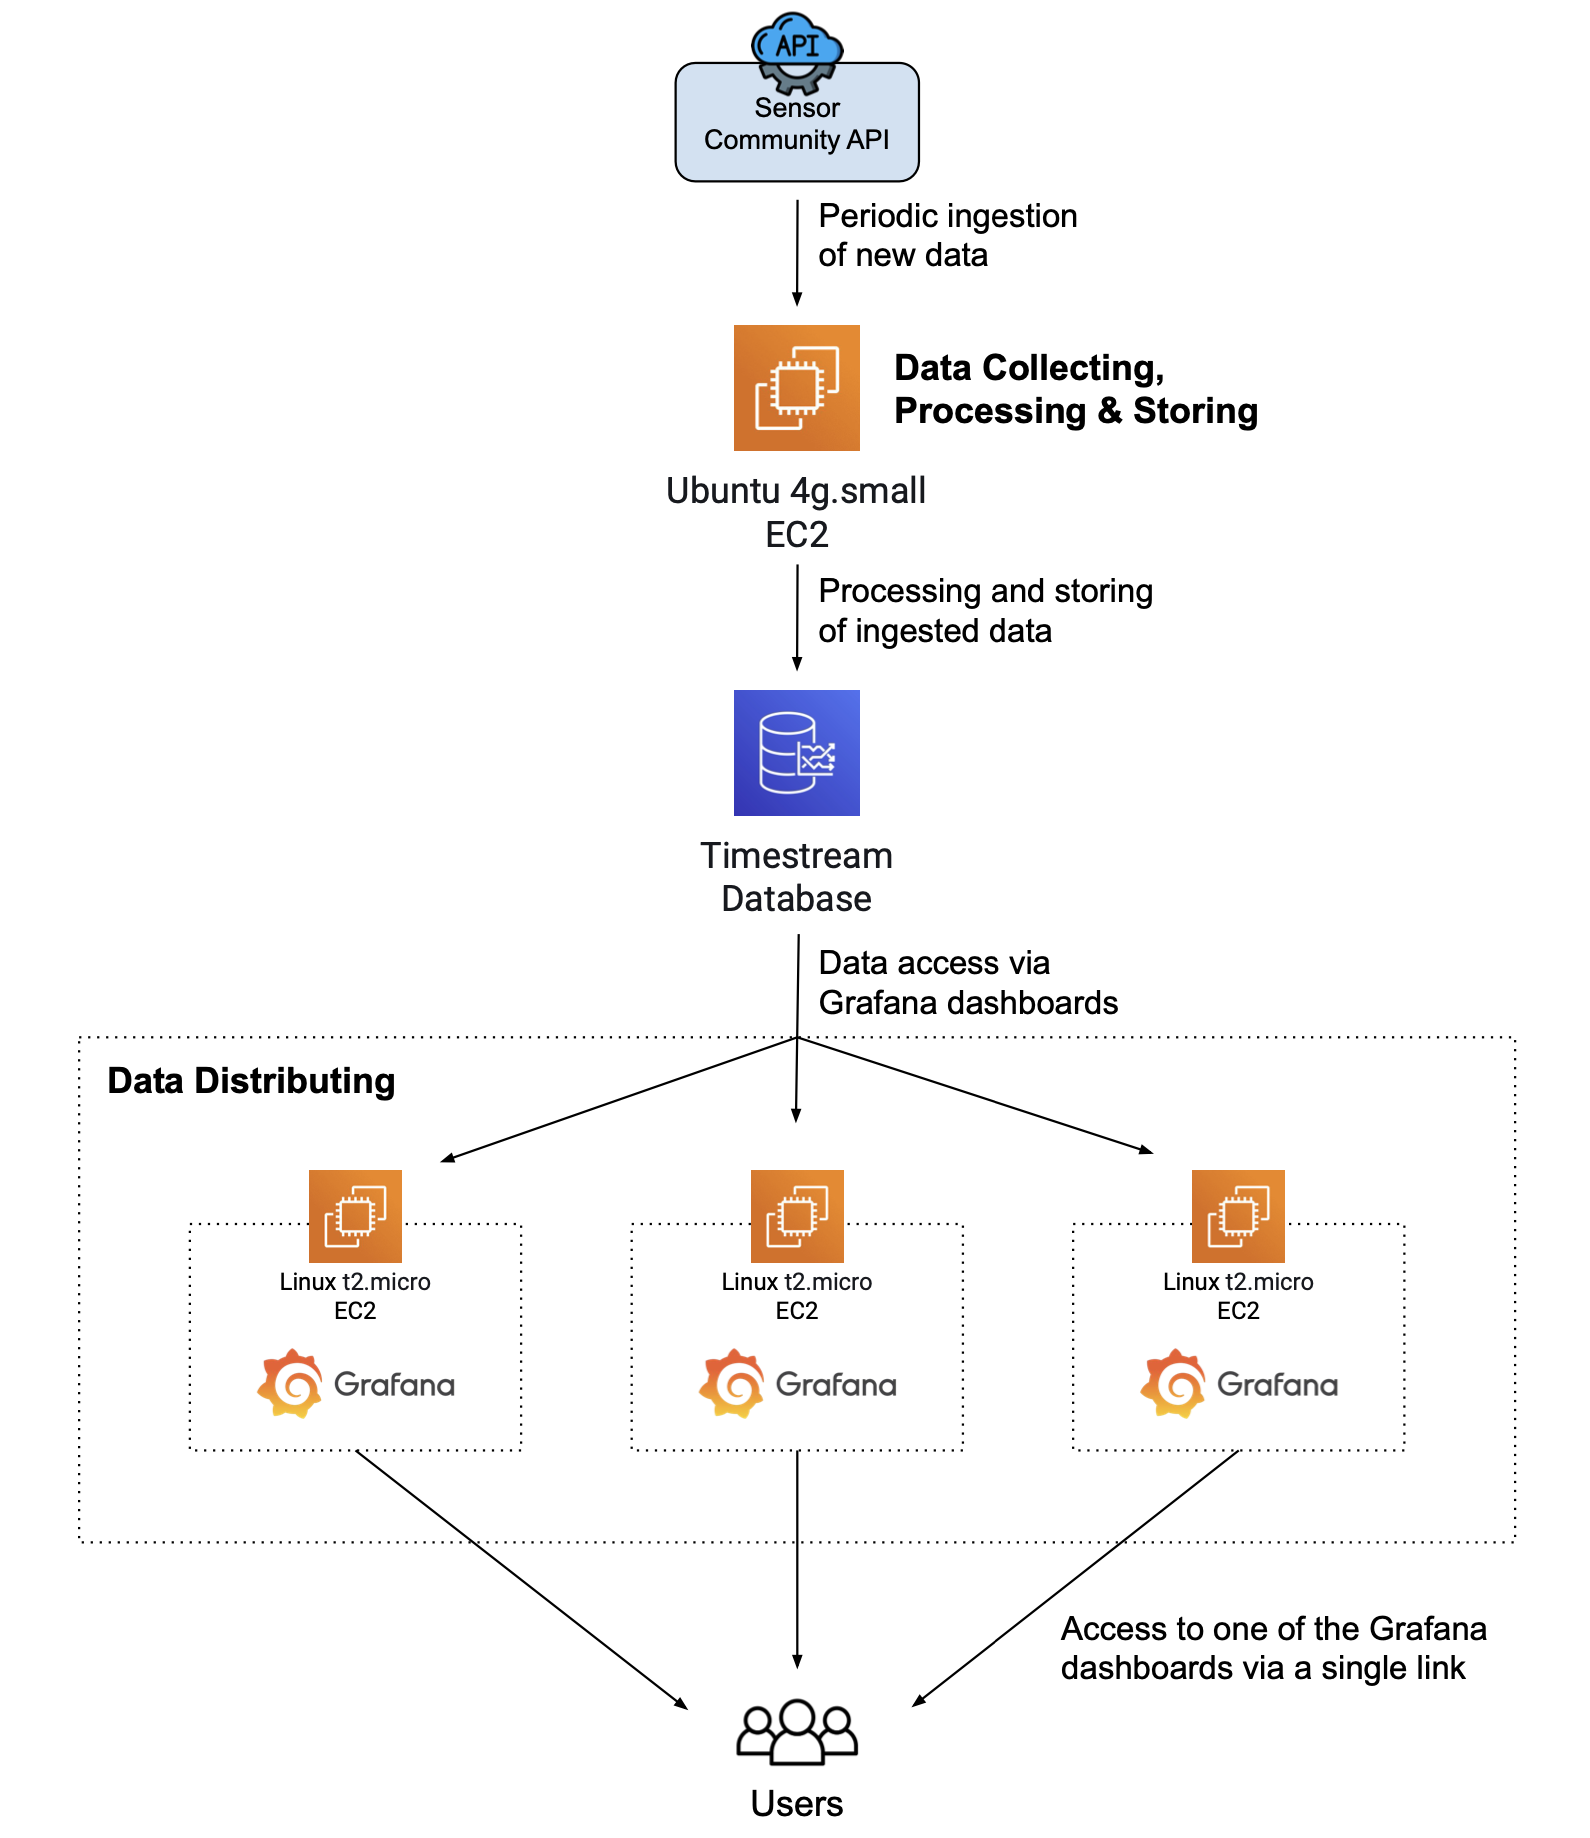
\includegraphics[width=1\linewidth]{images/pipeline.png}
    \caption{Project Architecture Diagram}\label{fig:project-pipeline}
\end{figure}

\newpage
\section{Data Collecting, Processing \& Storing}
\subsection{Overview of the first pipeline architecture}

In the \textbf{Data Collecting} phase, the last set of data is obtained from
its source, marking the start of the data pipeline. Following this, the
\textbf{Data Processing} phase takes over, where the data undergoes formatting
and calculation of the Air Quality Index (AQI) for each particulate matter
sensor. The final phase, \textbf{Data Storing}, involves meticulous storage of
data from each sensor in a time-series database.

For a detailed visual representation of this pipeline, refer to
Figure~\ref{fig:data-collecting-processing-storing-pipeline}, which illustrates
the Data Collecting, Processing, and Storing Pipeline.

\begin{figure}[H]
    \centering
    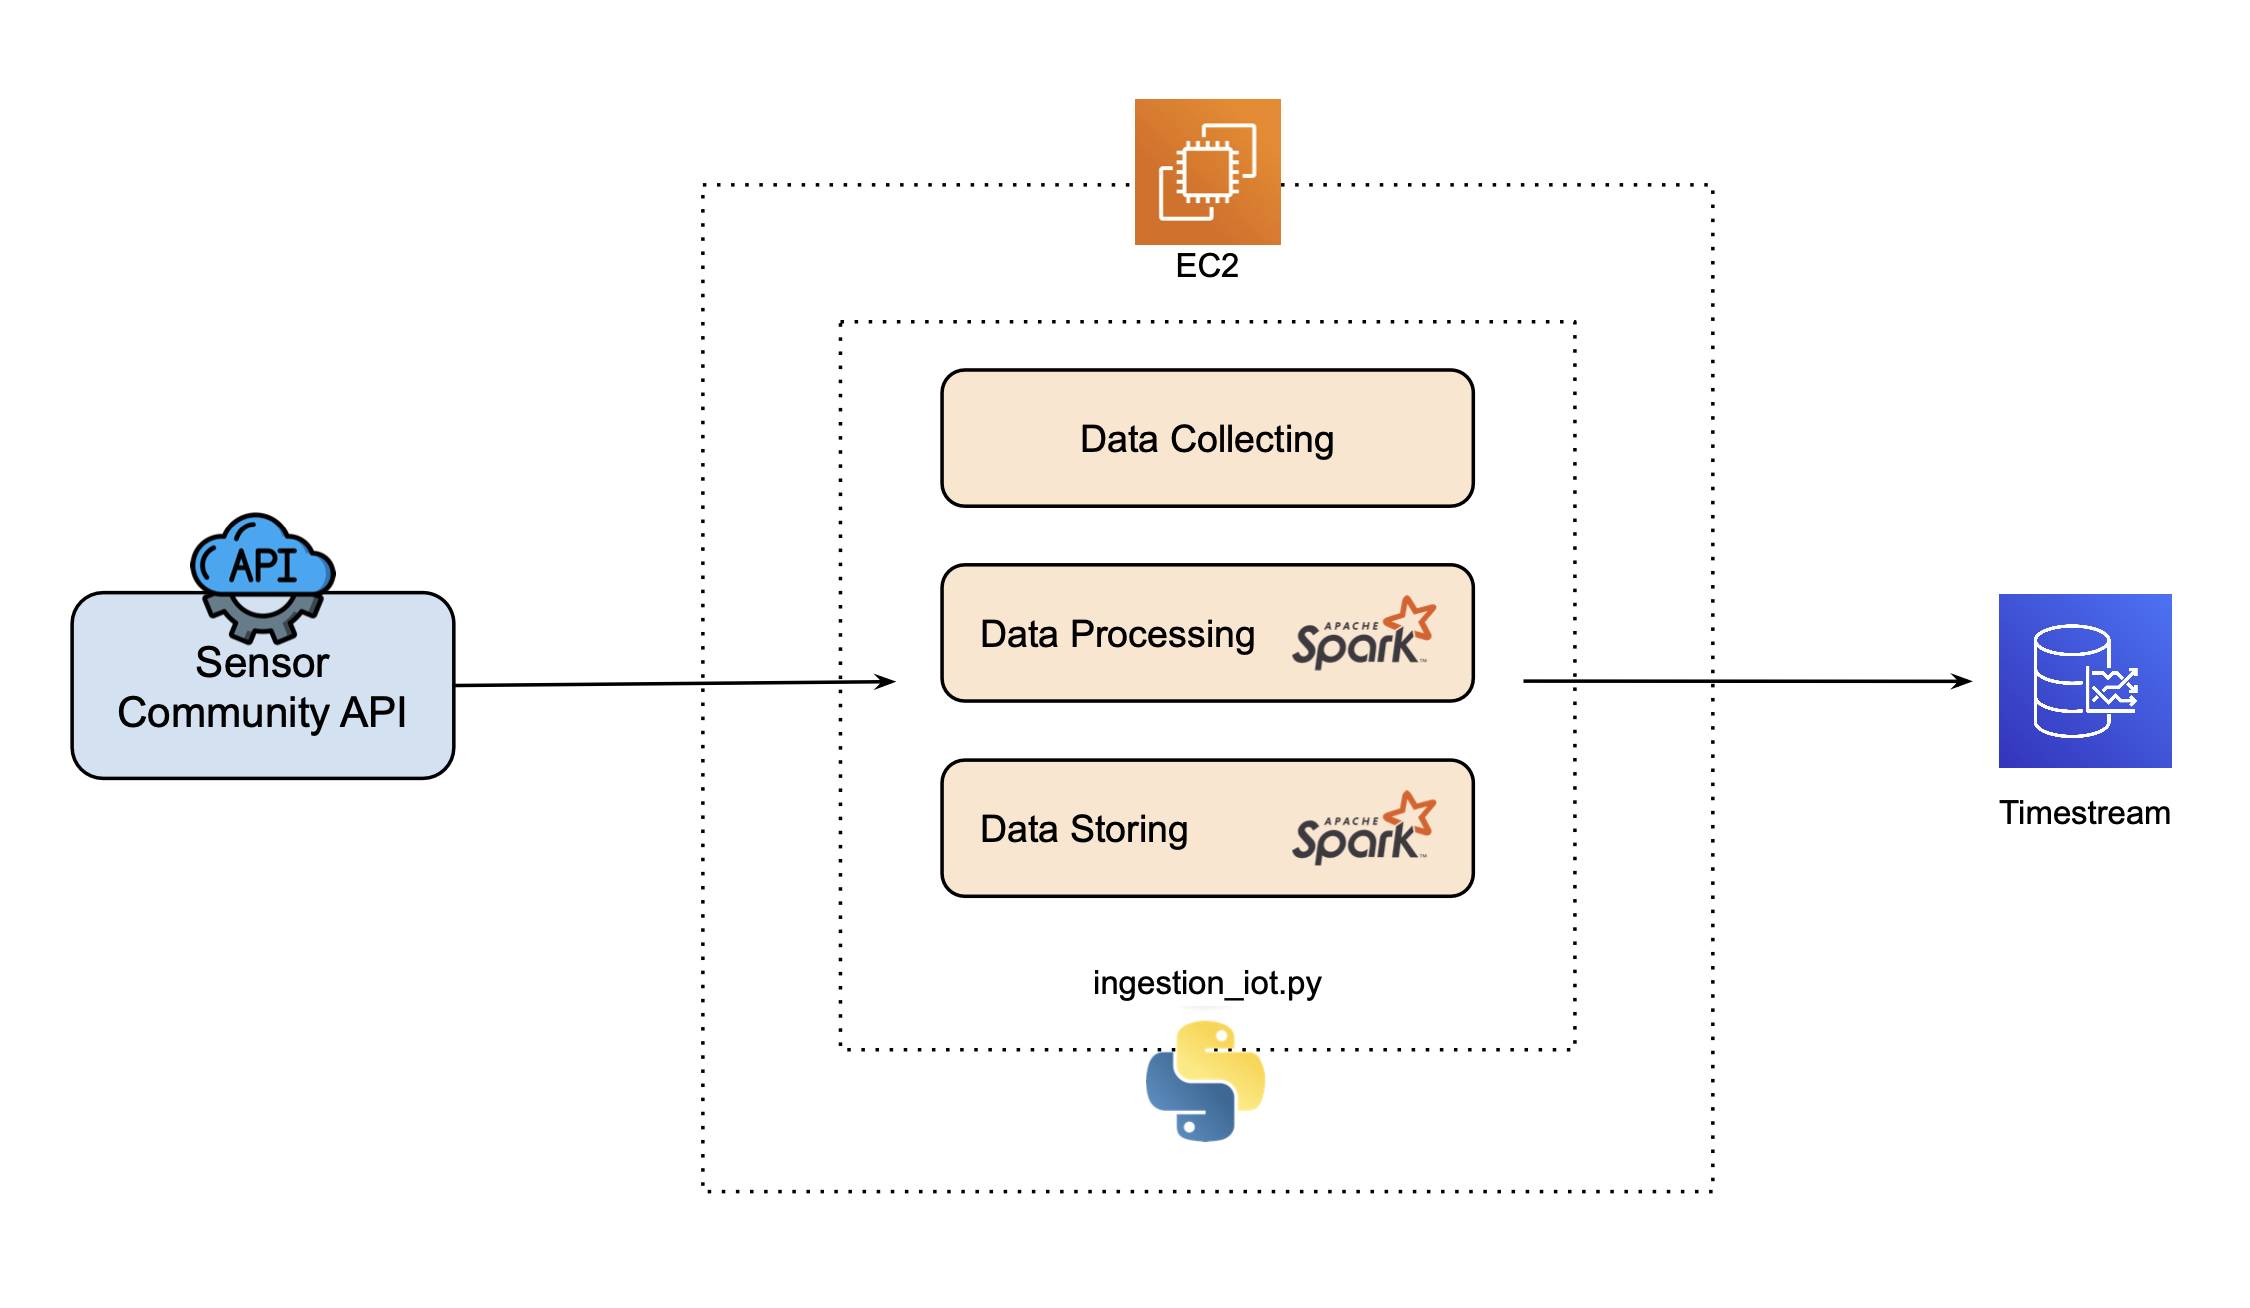
\includegraphics[width=1\linewidth]{images/cloud-computing-data-ingestion.png}
    \caption{Data Collecting, Processing \& Storing Pipeline Diagram}\label{fig:data-collecting-processing-storing-pipeline}
\end{figure}

\subsection{Data Collecting}
\subsubsection{Data Source}
The Sensor Community network is a global, contributor-driven initiative that
collects open environmental data through a vast network of sensors. These
sensors, deployed in over 70 countries, collect real-time data on air quality,
temperature, humidity and pressure. On average, the sensors send new data every
145 seconds~\cite{sensorcommunity2023synchronization}. The Sensor Community
network offers two main API endpoints for accessing their environmental data:

\begin{enumerate}
    \item \textbf{5-Minute Averaged Data API:} This API provides data averaged over the last 5 minutes for each sensor.
    \item \textbf{24 Hour Averaged Data API:} This API provides data averaged over the last 24 hours for each sensor.
\end{enumerate}

\subsubsection{Ingestion Script}
The data acquisition process in this project involved leveraging both APIs from
the Sensor Community. To do this, the Python \texttt{Requests} library was
used, enabling efficient data retrieval. Once collected, the data is
temporarily stored in a local cache, formatted as a Spark DataFrame for
optimised handling and processing. This operation, executed by the
\texttt{fetch\_sensors\_data} function, is located within the
\texttt{collecting.py} script (see Appendix~\ref{appendix:collecting} for
detailed code). In particular, this function is programmed to run at a constant
interval of 10 seconds, ensuring a regular and up-to-date flow of data from the
sensors.

\subsection{Data Processing}

\subsubsection{Processing Script}
The data processing stage initiates with the activation of the
\texttt{computeAQI} function, following data ingestion. This crucial function
uses user-defined functions (UDFs) to convert PM2.5 and PM10 concentration data
into Air Quality Index (AQI) values, adhering to the guidelines specified in
Table~\ref{tab:uk_aqi}. The comprehensive implementation details of this
function are available in the \texttt{processing.py} script, as detailed in
Appendix~\ref{appendix:processing}.

Key to this stage is the utilisation of Spark DataFrames, which offer an
efficient means of managing and processing the data due to their distributed
structure. The data is first restructured using the \texttt{explode} operation,
which separates each sensor's data into individual rows, thus preparing it for
the application of UDFs. To enhance efficiency, the DataFrame is then cached,
significantly reducing the need for repetitive disk read/write operations and
thereby accelerating the computation process.

\begin{table}[H]
    \centering
    \caption{UK air quality index, ``Review of the UK Air Quality Index'', 2011}
    \begin{tabular}{|p{2cm}|p{2cm}|p{3,5cm}|p{3,5cm}|}
        \hline
        \textbf{Range} & \textbf{Air Quality Index} & \textbf{PM\(_{2.5}\) Particles, 24 hour mean (\(\mu g/m^3\))} & \textbf{PM\(_{10}\) Particles, 24 hour mean (\(\mu g/m^3\))} \\ \hline
        Low            & 1                          & 0-11                                                          & 0-16                                                         \\
                       & 2                          & 12-23                                                         & 17-33                                                        \\
                       & 3                          & 24-35                                                         & 34-50                                                        \\ \hline
        Medium         & 4                          & 36-41                                                         & 51-58                                                        \\
                       & 5                          & 42-47                                                         & 59-66                                                        \\
                       & 6                          & 48-53                                                         & 67-75                                                        \\ \hline
        High           & 7                          & 54-58                                                         & 76-83                                                        \\
                       & 8                          & 59-64                                                         & 84-91                                                        \\
                       & 9                          & 65-70                                                         & 92-100                                                       \\ \hline
        Very High      & 10                         & $>$70                                                         & $>$100                                                       \\ \hline
    \end{tabular}
    \label{tab:uk_aqi}
\end{table}

\subsubsection{Leveraging Apache Spark}
Apache Spark is a distributed computing framework that excels at managing and
processing large-scale data sets. Using Apache Spark improves data processing
capabilities in several ways:

\begin{enumerate}
    \item \textbf{Scalability for Varying Data Volumes:} Apache Spark's scalable architecture is optimally designed to handle the varying volumes and complexity of IoT sensor data. This scalability is crucial for real-time data processing, ensuring fast and efficient AQI calculations.

    \item \textbf{Parallel processing between nodes:} The distributed nature of Spark enables parallel processing of computational tasks across multiple nodes. This functionality is essential for the simultaneous processing of AQI calculations from a range of sensors, significantly increasing the speed and efficiency of data processing.
\end{enumerate}

\subsection{Data Storing}

\subsubsection{Database Choice}
The difficulty with this project lies in the efficient management of data
storage. Each sensor can measure a variety of data, making the structure of a
single relational database too complex and inefficient. This complexity
increases as the volume of data increases, requiring the creation of multiple
linked tables.

Faced with these challenges, time series databases (TSDBs) are emerging as an
optimal solution. Unlike traditional relational databases, TSDBs are
specifically designed to manage time-series data, such as that from IoT
sensors. They offer better performance in tracking, monitoring and aggregating
data over time.

Amazon Timestream is a good choice for this project. As a cloud-native
time-series database, it offers superior time-series management capabilities
tailored to IoT sensor data. What sets Amazon Timestream apart is the speed
with which it ingests data and its efficiency in processing large volumes of
data, enabling regular updates and in-depth analysis. Its ability to adapt to
changing workloads ensures consistent performance, a major advantage for
real-time data management.

\subsubsection{Storing Script}
The data storing process represents the final phase in the IoT data collecting
and processing pipeline. Once the AQI has been calculated, the data must be
stored efficiently and securely to allow subsequent analysis and real-time
consultation. The \texttt{storing.py} script (see
Appendix~\ref{appendix:storing} for detailed code) is designed to interact with
the Amazon Timestream database.

The \texttt{keepOnlyUpdatedRows} function is responsible for checking what data
is already in Timestream and keeping only the newly updated values. This
process begins by querying Timestream to retrieve the latest data timestamp for
each sensor using the `boto3` client. The data is then filtered to exclude
records that do not reflect new measurements, optimising storage space and
database performance.

Once this filtering is complete, the \texttt{writeToTimestream} function takes
over. It transforms each partition of the Spark DataFrame into a series of
structured records, containing the dimensions and measurements corresponding to
each sensor. These records are then written to Timestream in batches. The
process is carefully managed to ensure that records are written atomically and
consistently, with robust exception handling to deal with any rejected records.

\subsection{Pipeline Implementation on AWS}
Setting up an IoT data processing pipeline on Amazon Web Services (AWS)
involves several key steps, from configuring the EC2 instance to running and
managing the pipeline. The process is described below:

\begin{enumerate}
    \item \textbf{EC2 Instance Configuration:} A t4g.small EC2 instance with Ubuntu~\ref{fig:ec2-instance-configuration} has been configured to host the data collecting, processing \& storing pipeline. This type of instance was chosen for its balance between performance and energy efficiency. In addition, Apache Spark has been installed on this instance to process the data collected.
    \item \textbf{Setting Up Automated Services:} Two systemd services, which are activated each time the instance is started, were then set up to automate the following tasks:
          \begin{itemize}
              \item \textbf{get\_iam\_credentials.service:} This service (See Appendix~\ref{appendix:get-iam-credentials-service}) executes \texttt{get\_iam\_credentials.sh} (See Appendix~\ref{appendix:get-iam-credentials}). This script retrieves the instance's IAM credentials, enabling secure integration with other AWS services.
              \item \textbf{spark\_python\_job.service:} This service (See Appendix~\ref{appendix:spark-python-job-service}) launches \texttt{start\_spark\_job.sh} (See Appendix~\ref{appendix:start-spark-job}), which starts the script responsible for the collection, processing and storage of IoT data (See Appendix~\ref{appendix:main}).
          \end{itemize}
\end{enumerate}

\begin{figure}[H]
    \centering
    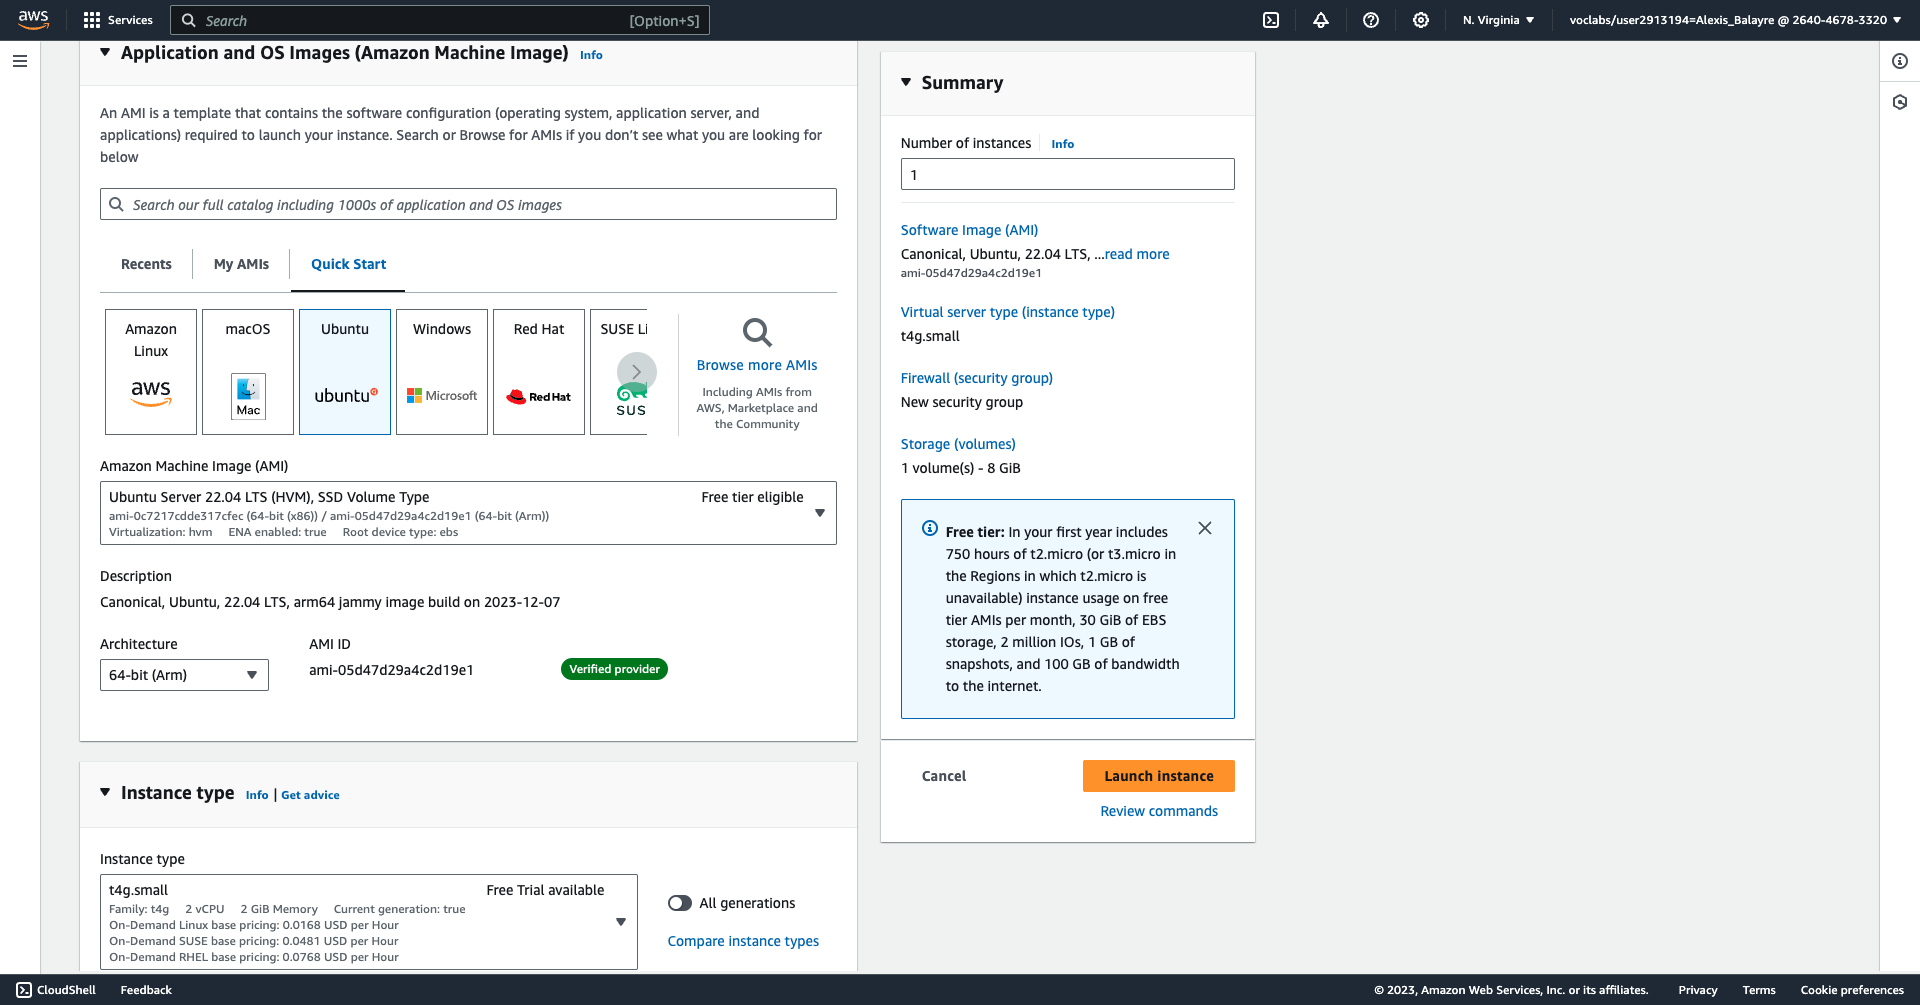
\includegraphics[width=1\linewidth]{images/t4g-small.png}
    \caption{EC2 Instance Configuration Screenshot}\label{fig:ec2-instance-configuration}
\end{figure}

\newpage
\section{Data Distributing}

\subsection{Overview of the second pipeline architecture}
The second pipeline of this project focuses on the efficient distribution and
monitoring of processed data, comprising several essential components:

\begin{enumerate}
    \item \textbf{Internet Gateway}: \\
          This is the entry point for user interaction, directing them to the Grafana dashboards through specific URLs.

    \item \textbf{Load Balancer}: \\
          Central to this pipeline, the Load Balancer evenly distributes the workload across EC2 instances.

    \item \textbf{Grafana Dashboard Access}: \\
          Hosted on EC2 instances, the Grafana dashboard provides an interactive platform for data visualization.

    \item \textbf{CloudWatch Monitoring}: \\
          AWS CloudWatch actively monitors system performance and dynamically adjusts resources to maintain system efficiency and stability.
\end{enumerate}

For a comprehensive visual overview of this pipeline, please refer to
Figure~\ref{fig:data-distributing-pipeline}, which depicts the Data
Distributing Pipeline.

\begin{figure}[H]
    \centering
    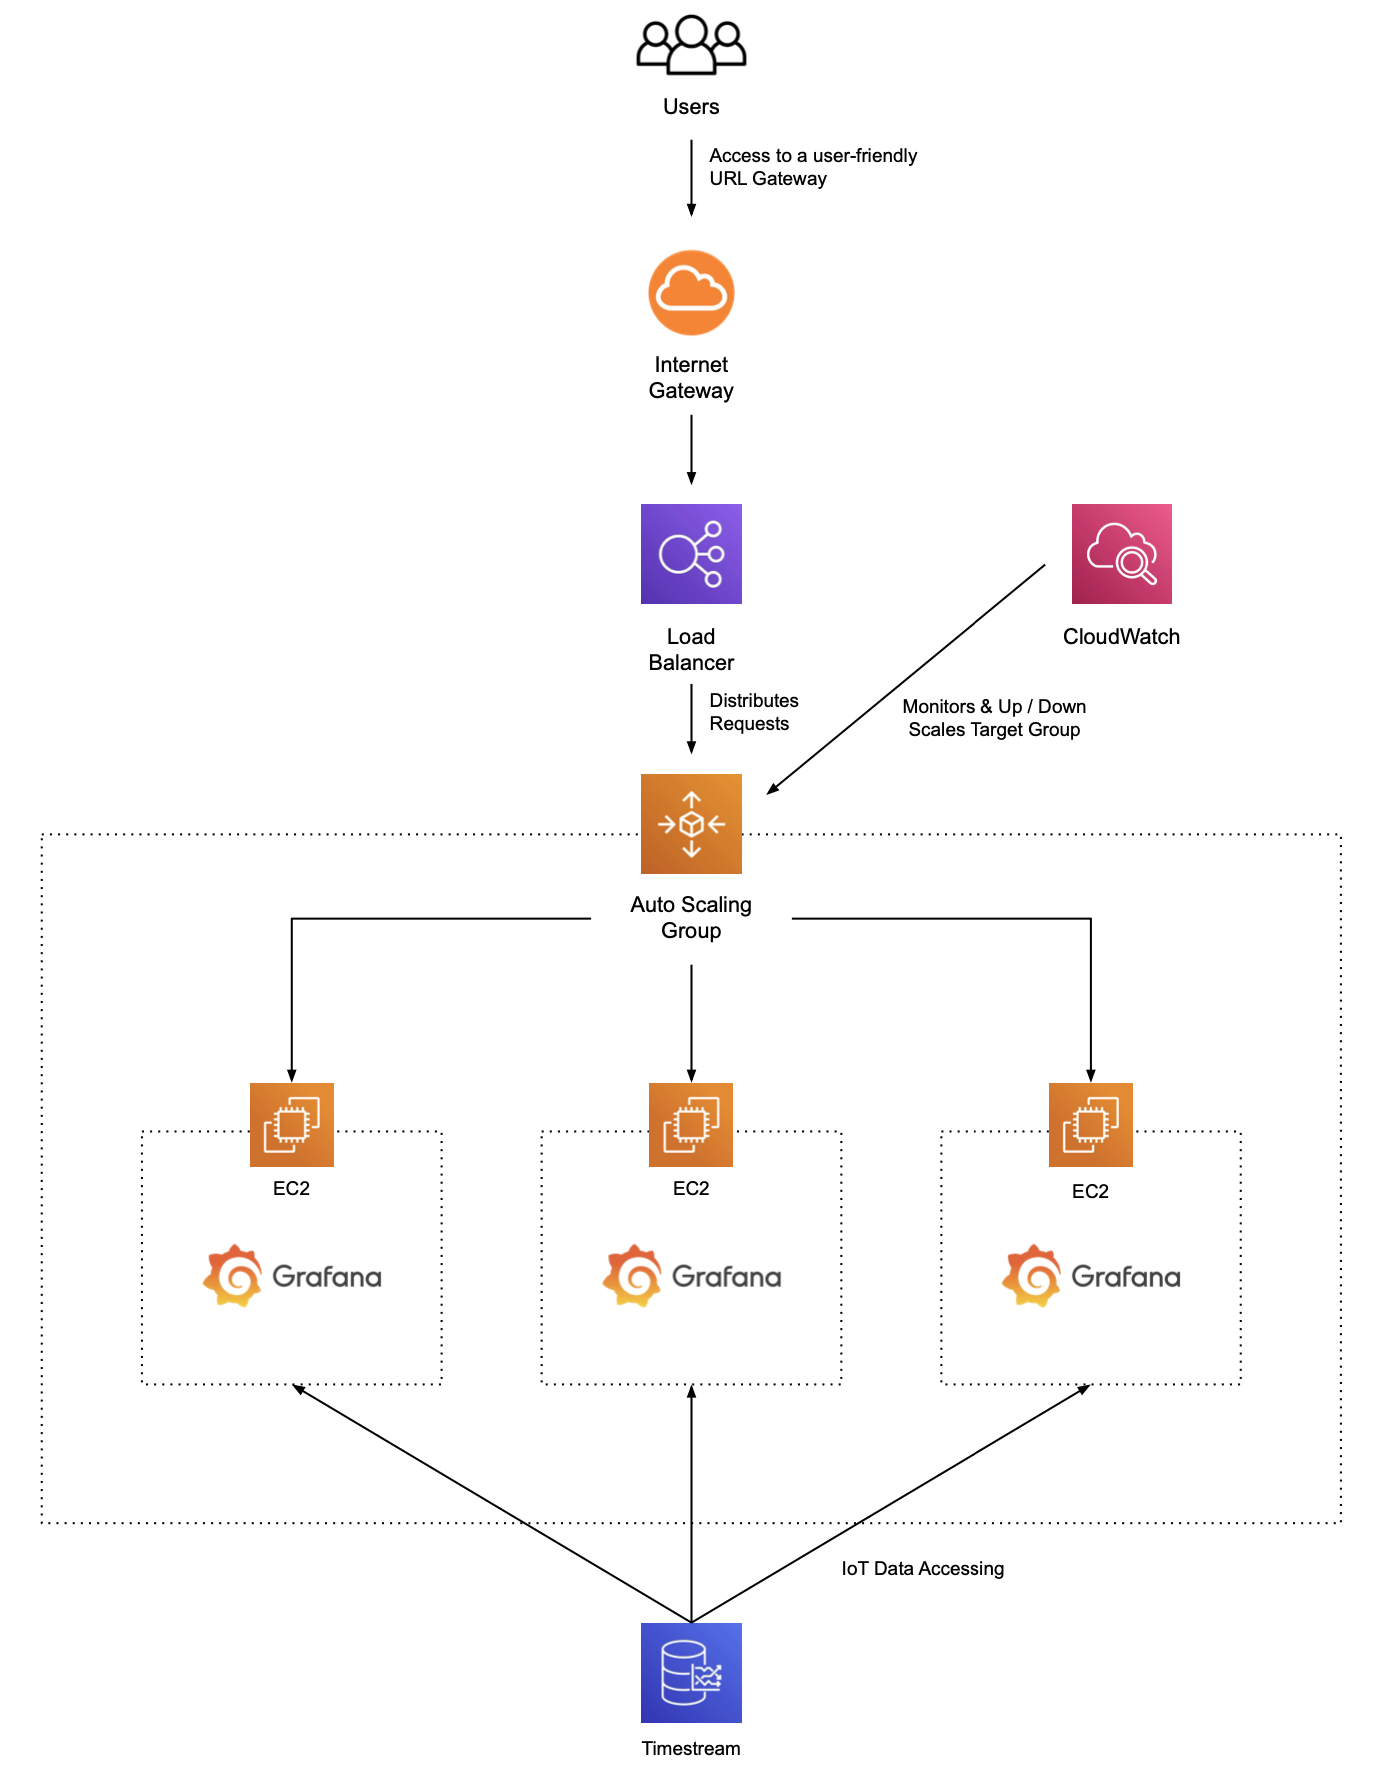
\includegraphics[width=1\linewidth]{images/cloud-computing-clients.png}
    \caption{Data Distributing Pipeline Diagram}\label{fig:data-distributing-pipeline}
\end{figure}

\newpage
\subsection{Auto Scaling Group Configuration}

The Auto Scaling Group plays a crucial role in dynamically managing the EC2
instances of the Data Distributing Pipeline. This section outlines the
configurations for the Auto Scaling Group and its associated components. The
figure below~\ref{fig:auto-scaling-group-pipeline} illustrates the Auto Scaling
Group Pipeline.

\begin{figure}[H]
    \centering
    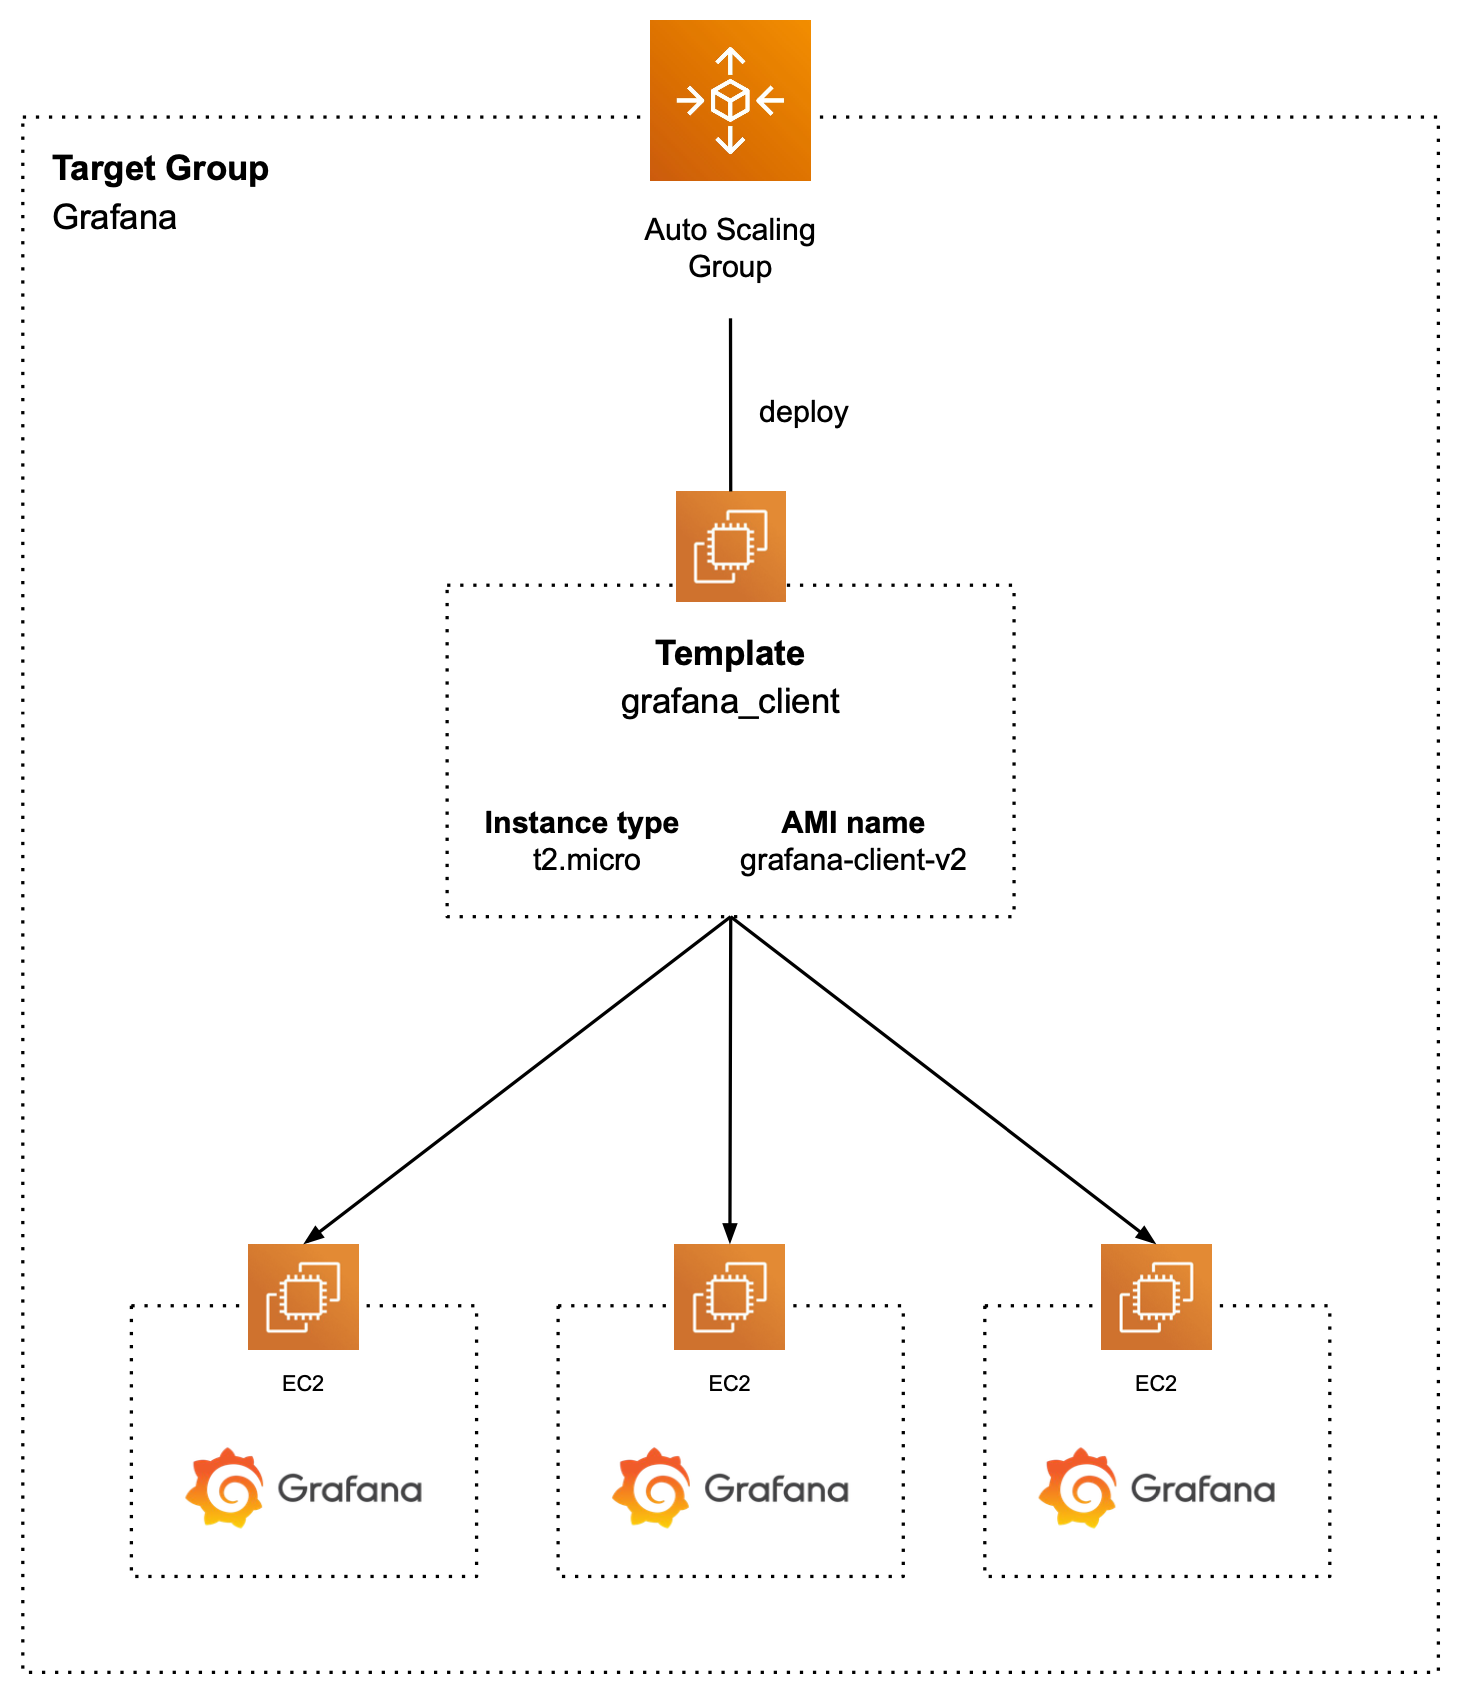
\includegraphics[width=1\linewidth]{images/grafana.png}
    \caption{Auto Scaling Group Pipeline Diagram}\label{fig:auto-scaling-group-pipeline}
\end{figure}

\newpage
\subsubsection{AMI Configuration}
An Amazon Machine Image (AMI) serves as a blueprint for launching an EC2
instance, containing the necessary software configuration. For this project, a
custom AMI was created using the Amazon Linux 2 operating system. A Grafana
server was configured on the AMI to display the IoT data in a user-friendly
format. The AMI was then stored in the AWS Elastic Block Store (EBS) for future
use.
\begin{figure}[H]
    \centering
    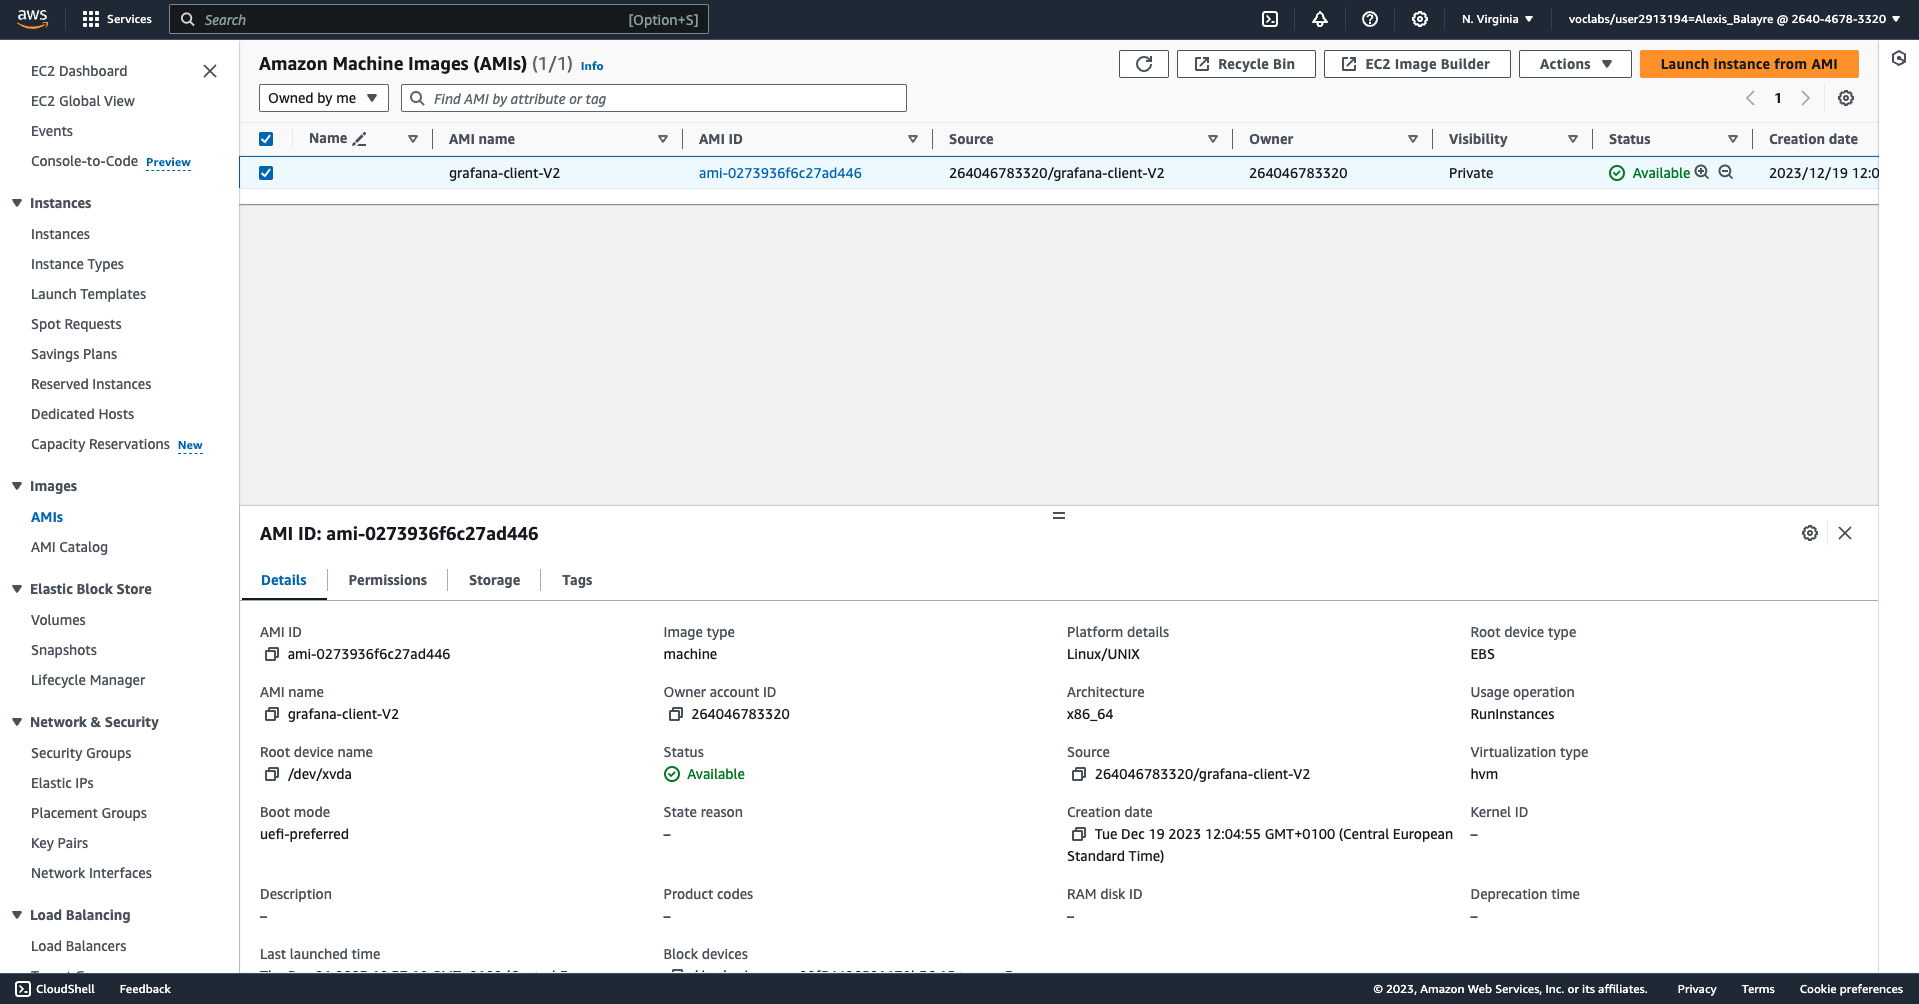
\includegraphics[width=1\linewidth]{images/ami.png}
    \caption{AMI Settings Screenshot}\label{fig:ami-settings}
\end{figure}

\newpage
\subsubsection{Launch Template Configuration}
The launch template defines the specifications for deploying EC2 instances
within the Auto Scaling Group. It incorporates the custom AMI and delineates
instance type, security group, key pair, and user data. This template deploys
t2.micro instances, which are ideal for light workloads, such as hosting the
Grafana server.
\begin{figure}[H]
    \centering
    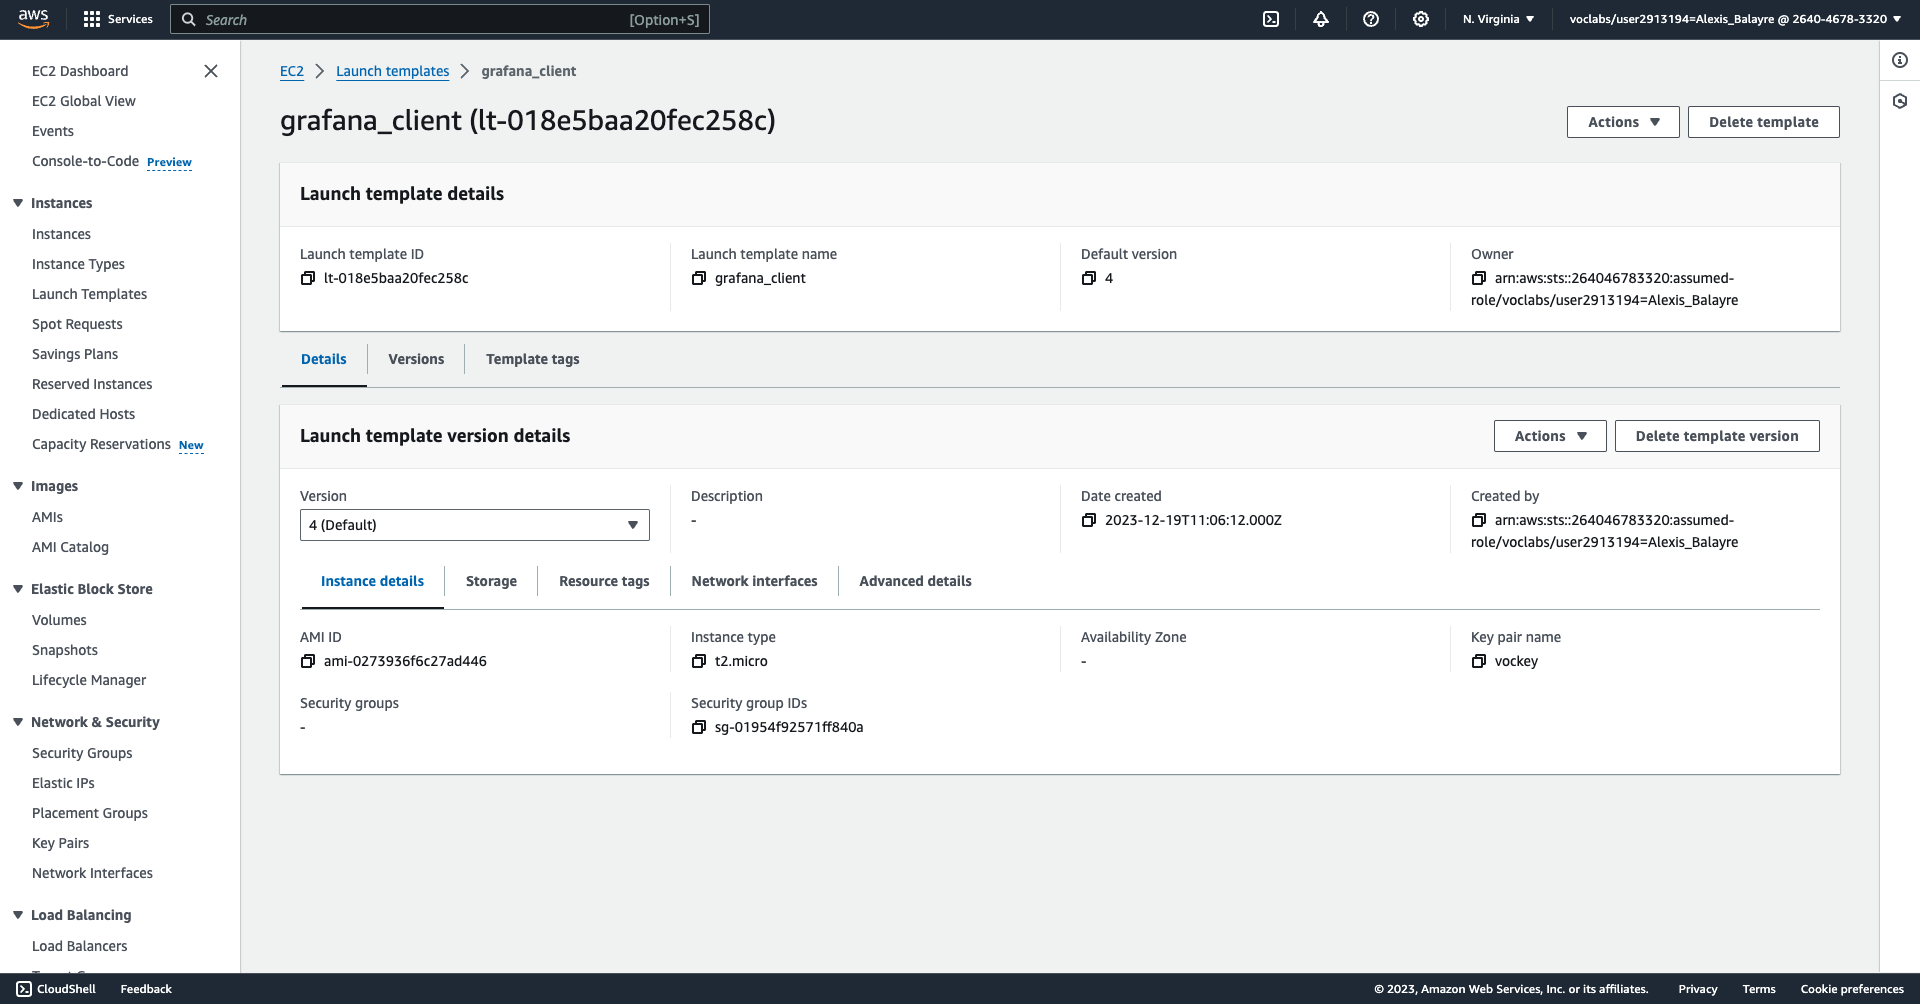
\includegraphics[width=1\linewidth]{images/launch-template.png}
    \caption{Launch Template Settings Screenshot}\label{fig:launch-template-settings}
\end{figure}

\newpage
\subsubsection{Auto Scaling Group Configuration}
The Auto Scaling Group is configured to automatically adjust the number of EC2
instances in response to the changing demand. It scales between 1 and 5
instances based on CPU utilisation, enhancing the system's responsiveness and
efficiency.
\begin{figure}[H]
    \centering
    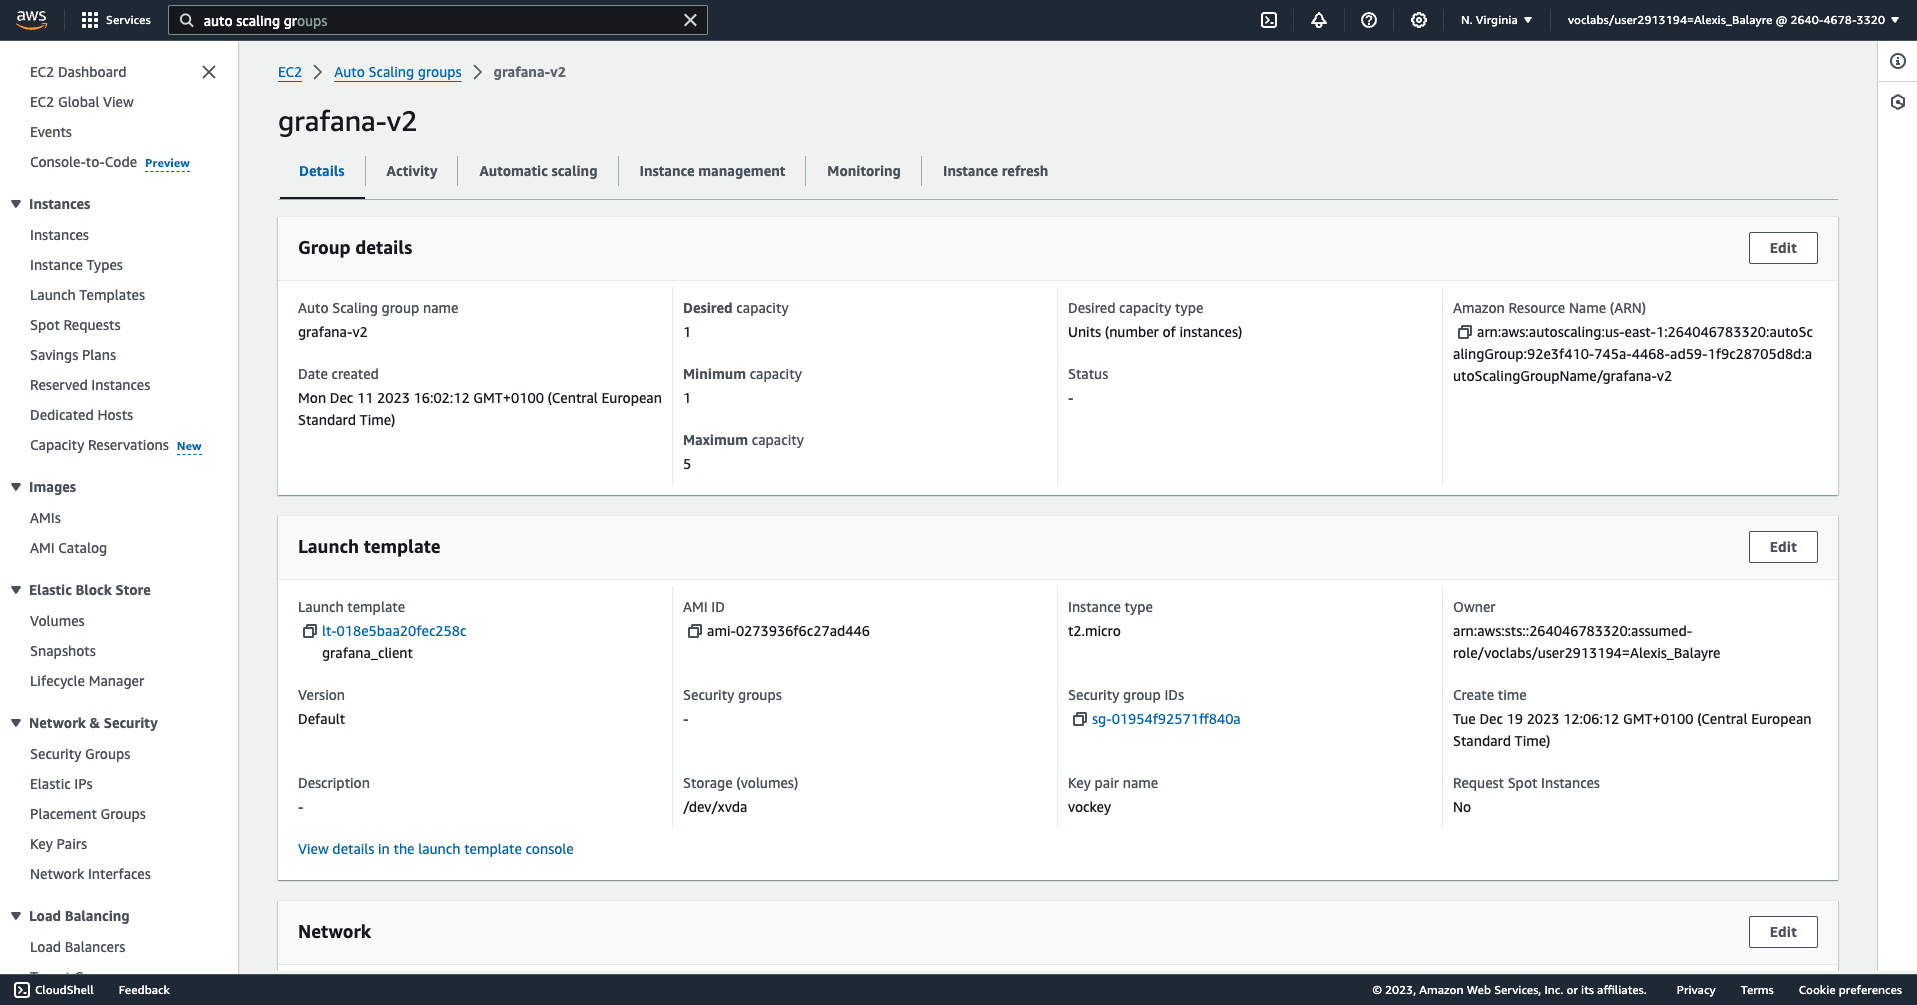
\includegraphics[width=1\linewidth]{images/auto-scaling-group.png}
    \caption{Auto Scaling Group Settings Screenshot}\label{fig:auto-scaling-group-settings}
\end{figure}

The Auto Scaling Group employs the following policies for scaling:
\begin{itemize}
    \item \textbf{Scale-out Policy:} Activates when average CPU utilisation exceeds 60\% for 3 minutes, adding an instance to the group.
    \item \textbf{Scale-in Policy:} Triggers when average CPU utilisation drops below 42\% for 15 minutes, removing an instance.
    \item \textbf{Cooldown Period:} Set at 150 seconds to maintain stability by preventing frequent scaling.
\end{itemize}

\begin{figure}[H]
    \centering
    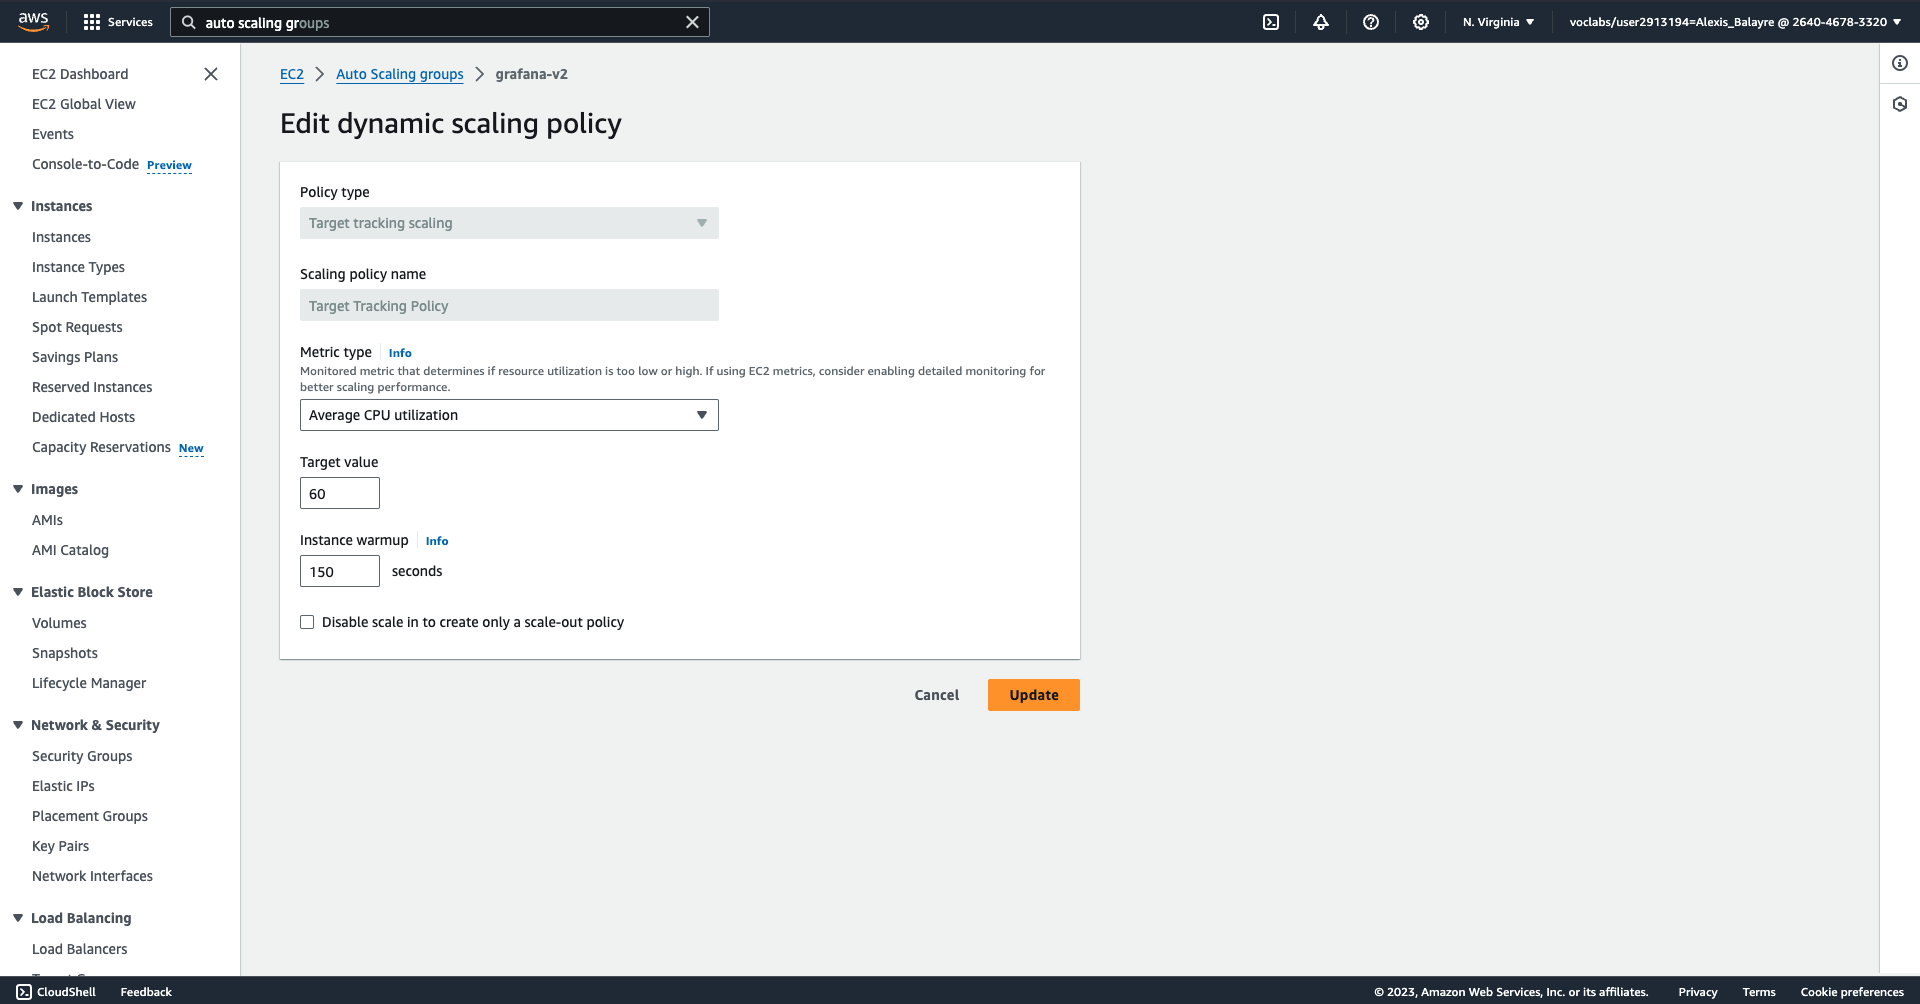
\includegraphics[width=1\linewidth]{images/scaling-policy.png}
    \caption{Scaling Policy Settings Screenshot}\label{fig:scaling-policy-settings}
\end{figure}

\subsubsection{Target Group Configuration}

A target group was created to distribute traffic between the EC2 instances of
the Auto Scaling Group.

\begin{figure}[H]
    \centering
    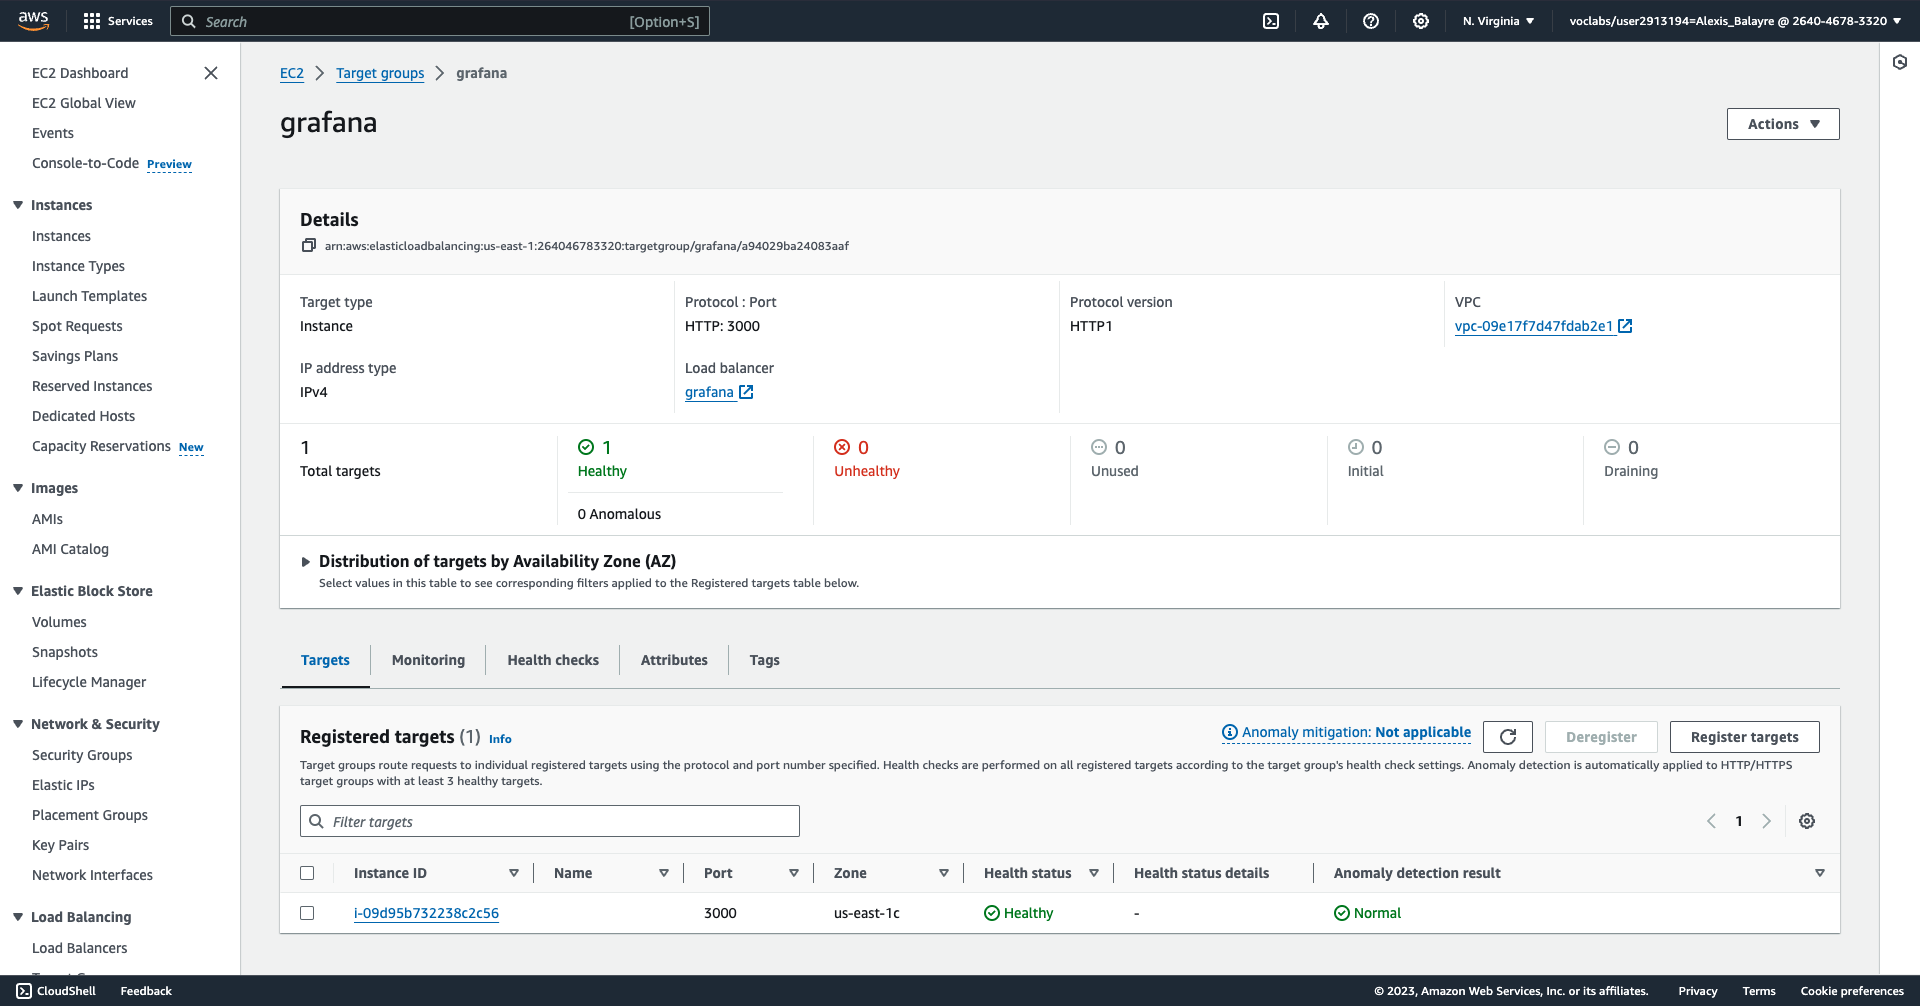
\includegraphics[width=1\linewidth]{images/target-group.png}
    \caption{Target Group Settings Screenshot}\label{fig:target-group-settings}
\end{figure}

\newpage
\subsubsection{Load Balancer Configuration}
A load balancer was created to distribute traffic between the EC2 instances of
the Auto Scaling Group. The load balancer is configured to use the target group
and to listen on port 80. This is useful for ensuring that the Grafana
dashboard is accessible to users through a user-friendly URL.
\begin{figure}[H]
    \centering
    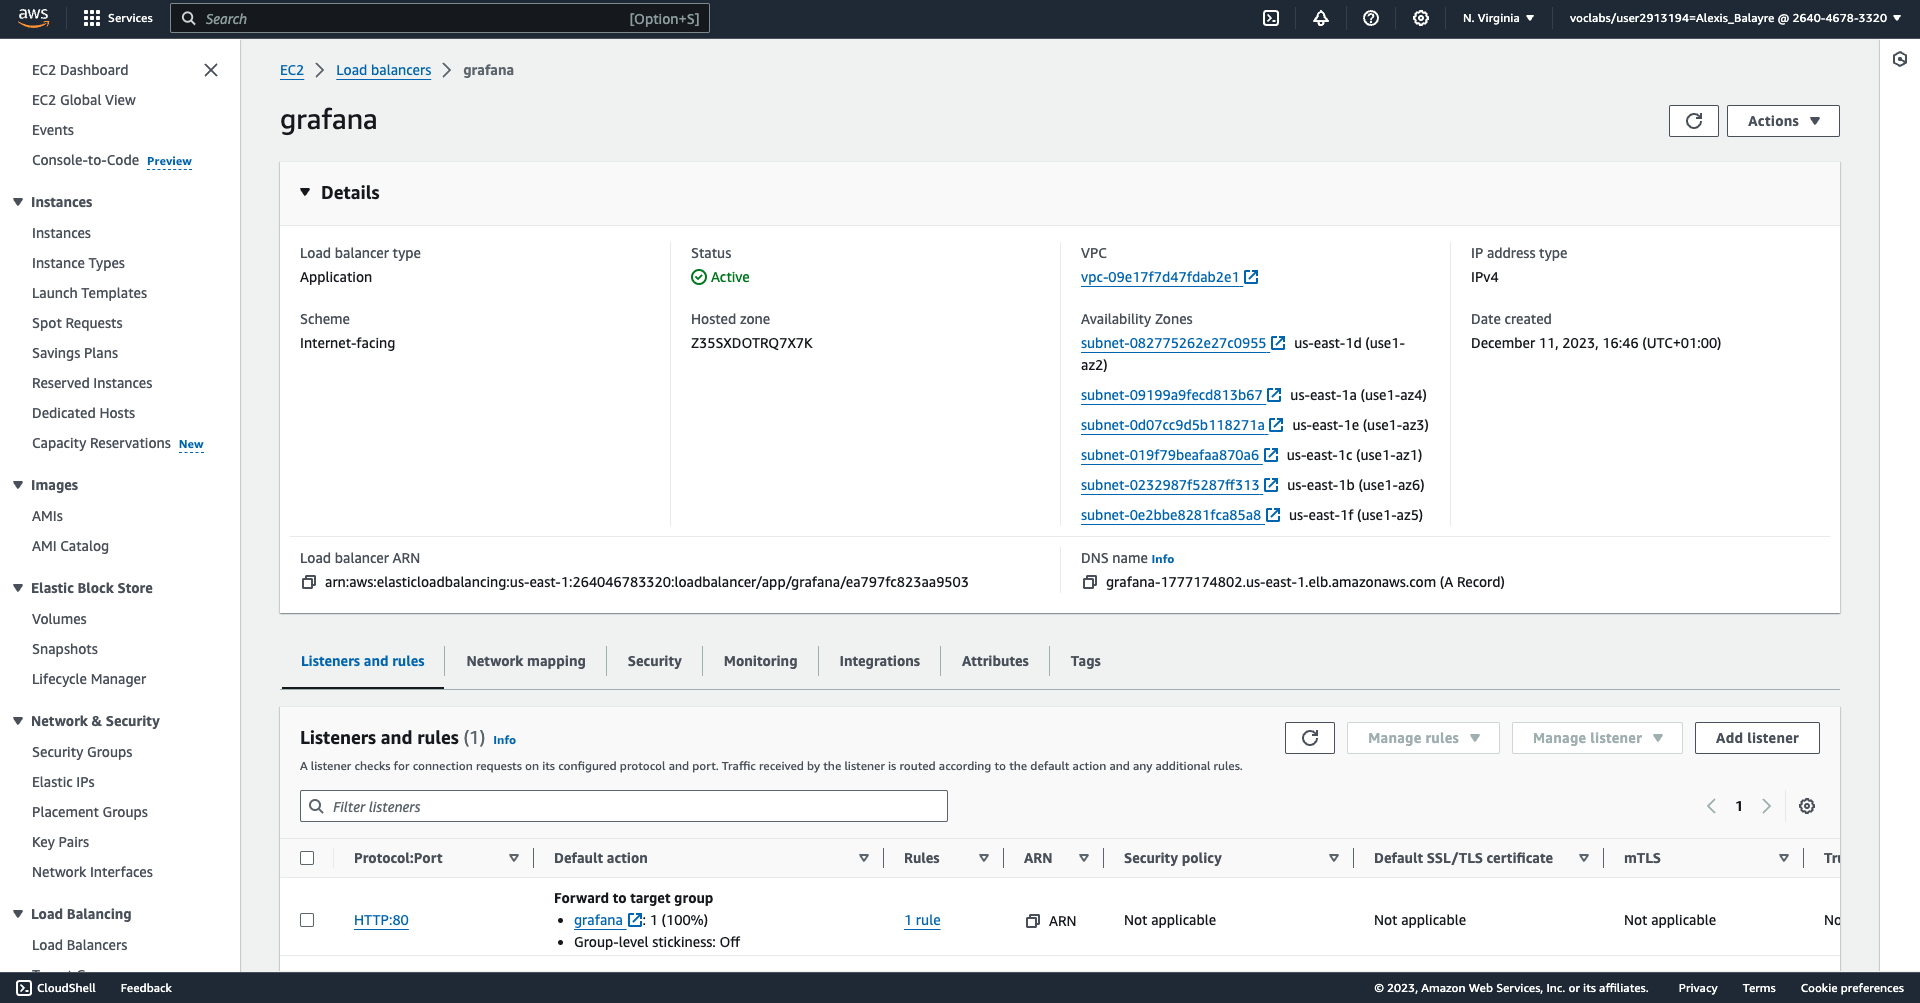
\includegraphics[width=1\linewidth]{images/load-balancer.png}
    \caption{Load Balancer Settings Screenshot}\label{fig:load-balancer-settings}
\end{figure}

\newpage
\chapter{Results \& Discussion}

\section{Results}
\subsection{Accessing the Data - Grafana Dashboard}

The Grafana dashboard provides an interactive interface enabling users to
analyse air quality data. It is accessible at the following URL:
\href{http://grafana-1777174802.us-east-1.elb.amazonaws.com/d/f8742187-f440-4ee8-96cc-bad5af8edef1/air-quality-monitoring}{Air
    Quality Monitoring Dashboard}. Users can customise the time interval,
measurement value and location ID. The dashboard consists of five main panels,
each providing unique information:
\begin{enumerate}
    \item \textbf{Measure Value Evolution:} This panel shows the evolution of the selected measure value in the selected location over the selected time range. This panel can be seen in Figure~\ref{fig:grafana-main-panel-1}.
    \item \textbf{Max AQI:} This panel shows the maximum AQI value in the selected location over the selected time range. This panel can be seen in Figure~\ref{fig:grafana-main-panel-1}.
    \item \textbf{Mean AQI:} This panel shows the mean AQI value in the selected location over the selected time range. This panel can be seen in Figure~\ref{fig:grafana-main-panel-1}.
    \item \textbf{AQI Map:} This panel shows the AQI value of each location on a map. This panel can be seen in Figure~\ref{fig:grafana-main-panel-2}.
    \item \textbf{IoT Data:} This panel shows all the data collected by the IoT sensors related to the selected measure value and time range. This panel can be seen in Figure~\ref{fig:grafana-main-panel-2}.
\end{enumerate}

\begin{figure}[H]
    \centering
    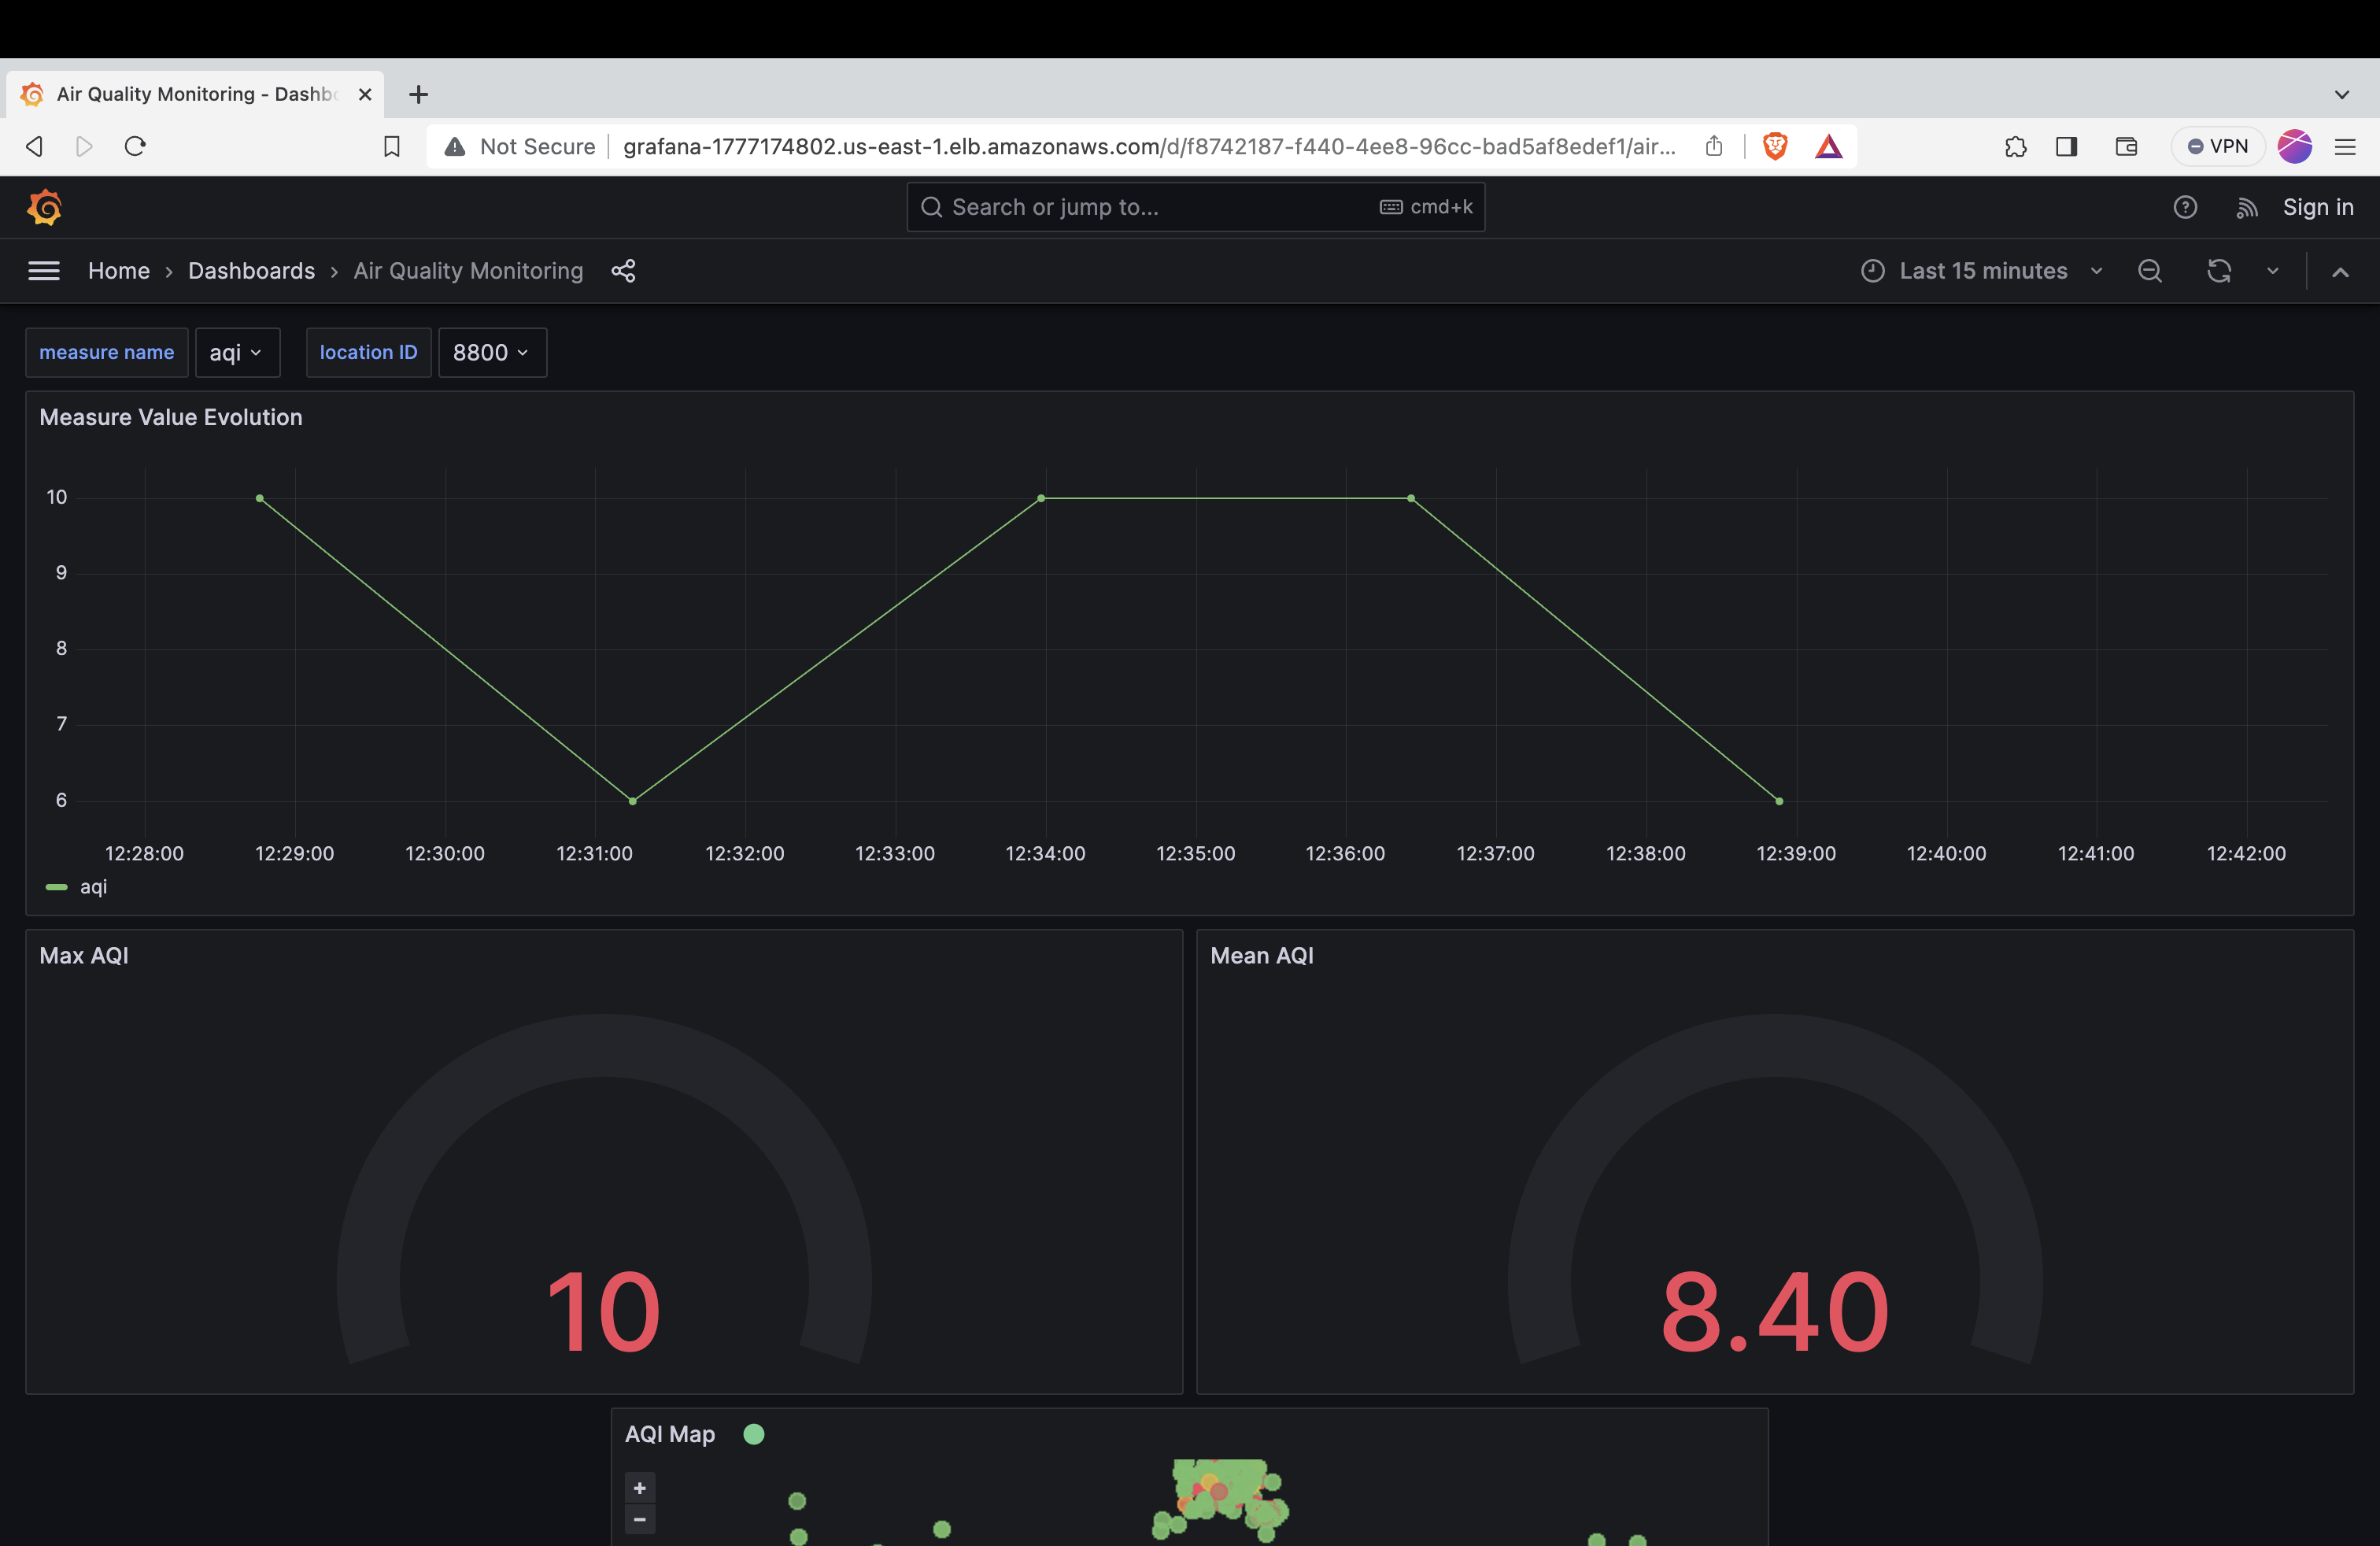
\includegraphics[width=1\linewidth]{images/grafana-1.png}
    \caption{Grafana Dashboard: Measure Value Evolution, Max \& Mean AQI}\label{fig:grafana-main-panel-1}
\end{figure}

\begin{figure}[H]
    \centering
    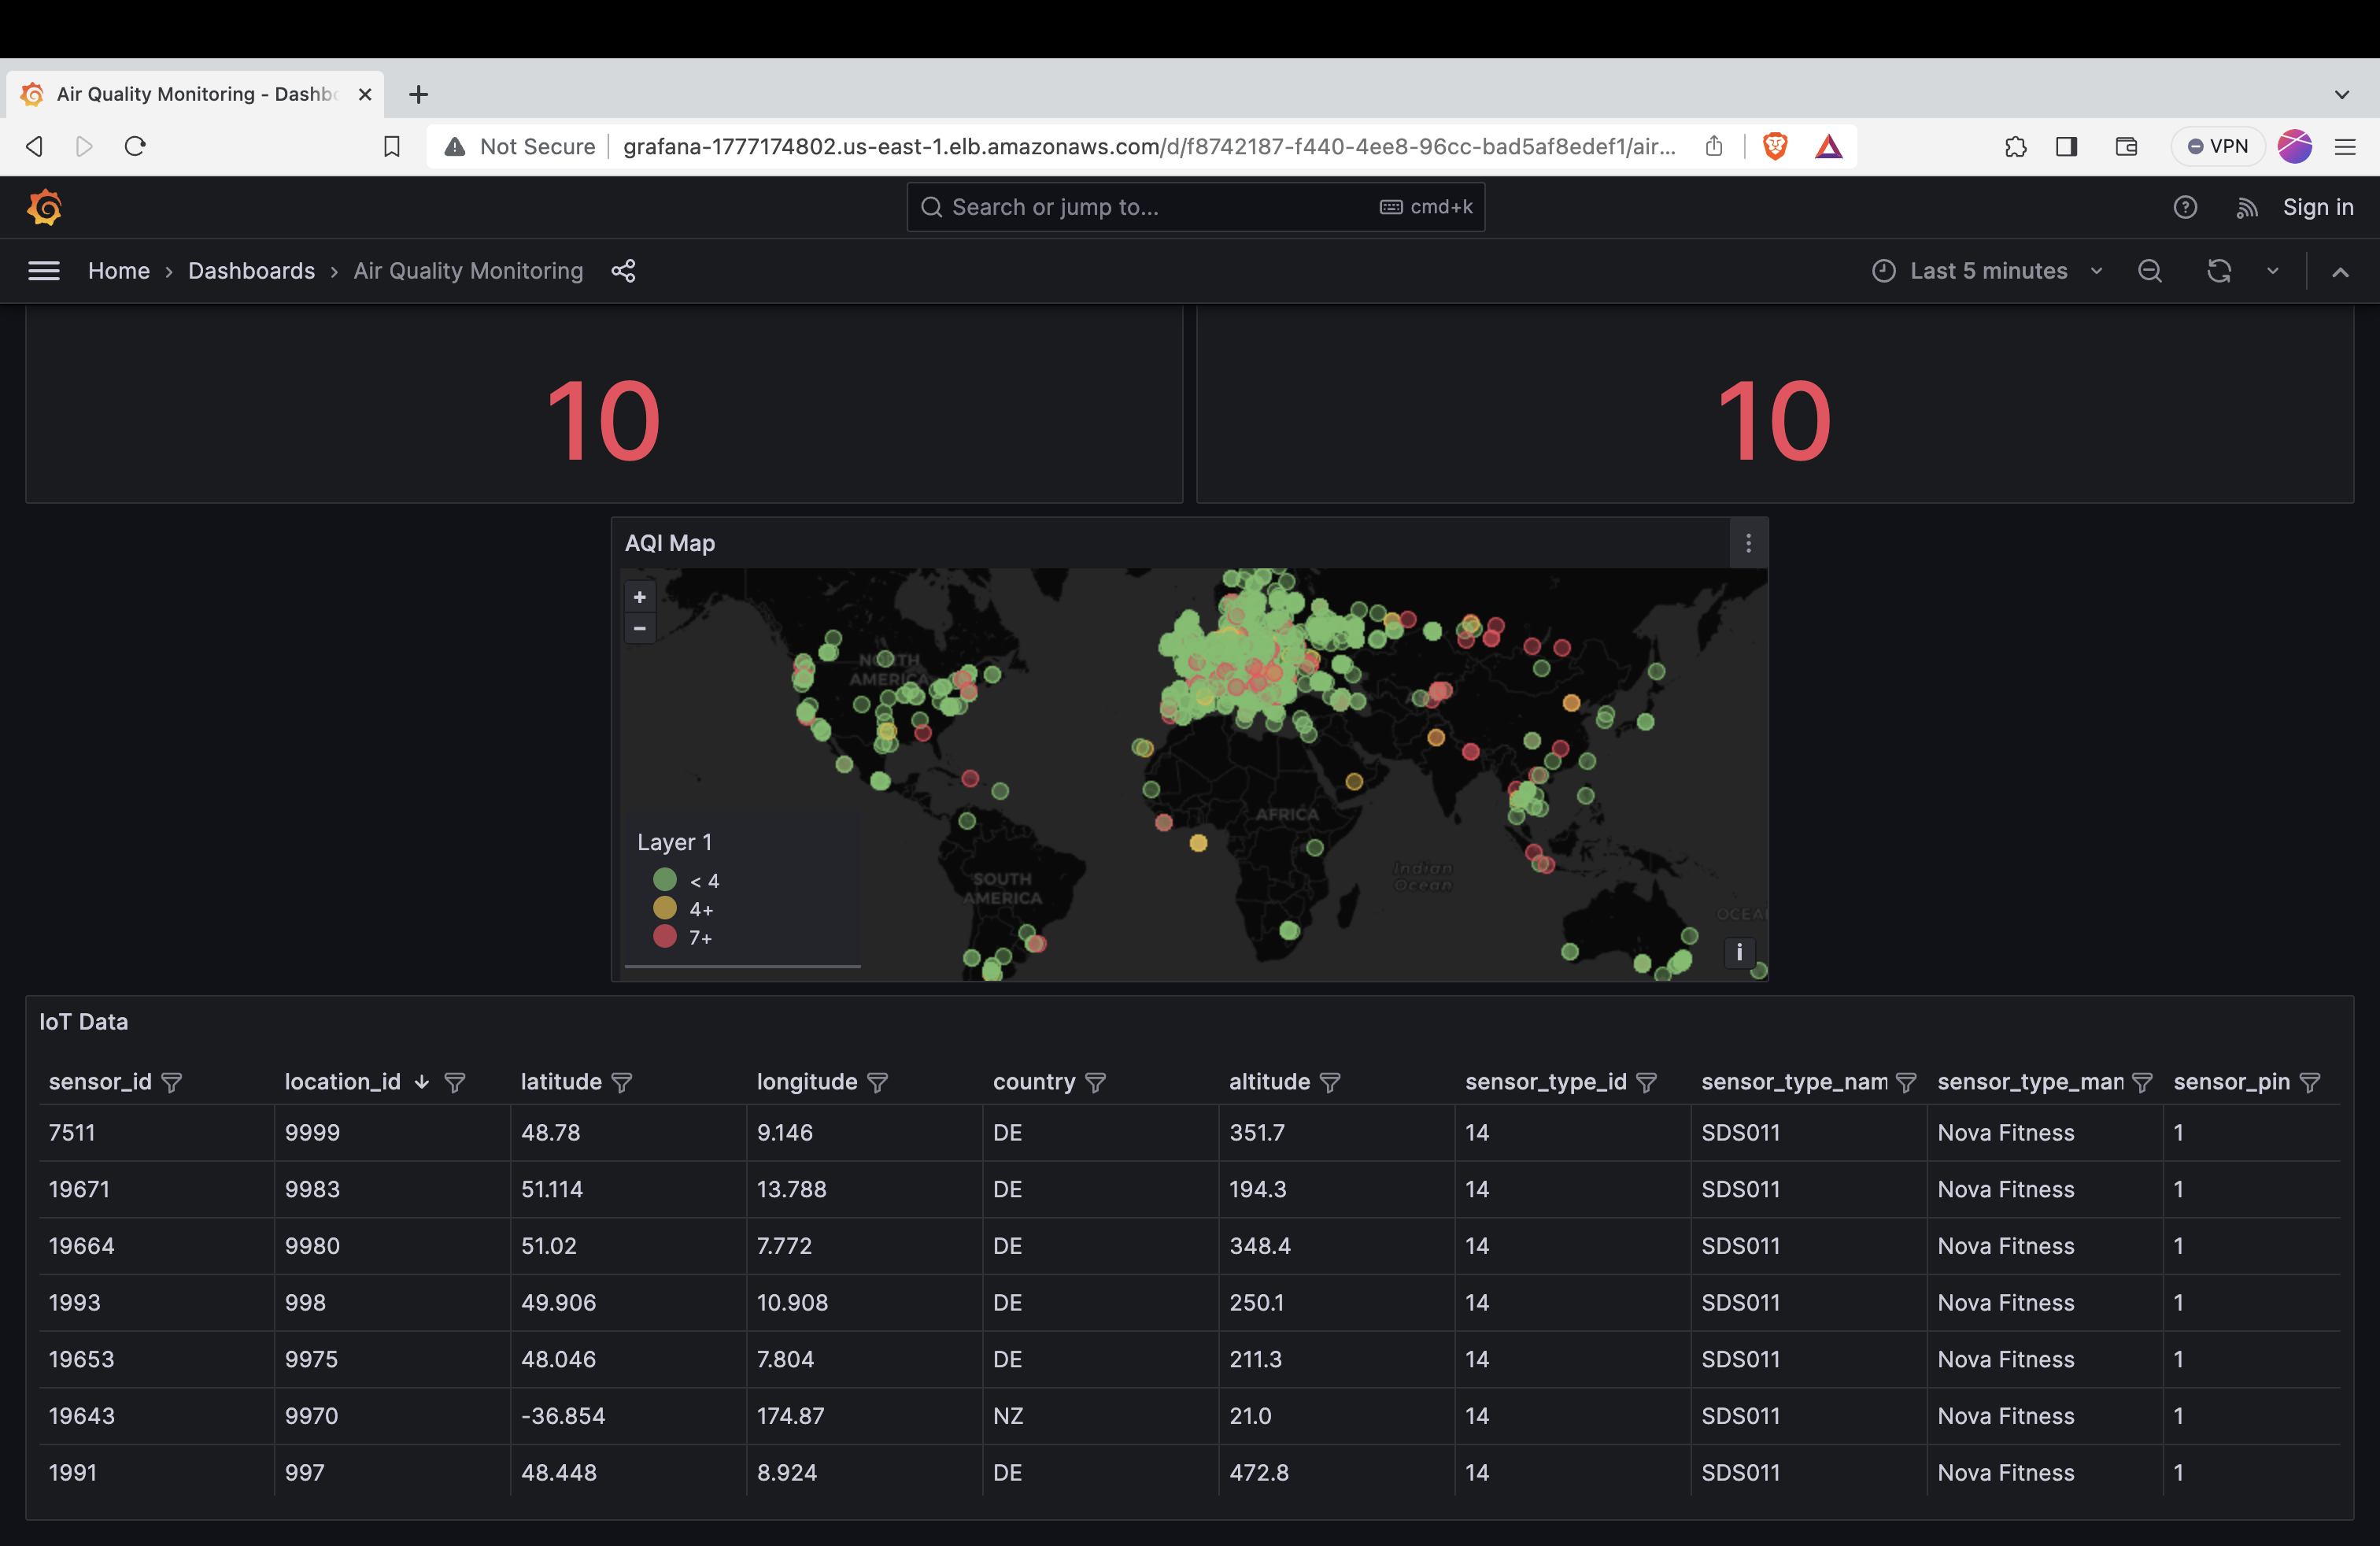
\includegraphics[width=1\linewidth]{images/grafana-2.png}
    \caption{Grafana Dashboard: AQI Map \& IoT Data}\label{fig:grafana-main-panel-2}
\end{figure}

\newpage
As shown in Figure~\ref{fig:grafana-aqi-map-panel}, the AQI Map panel displays
the AQI value of each location on a map. The AQI value is represented by a
colour, depending to the range it belongs to. The AQI value is also displayed
when hovering over a location.
\begin{figure}[H]
    \centering
    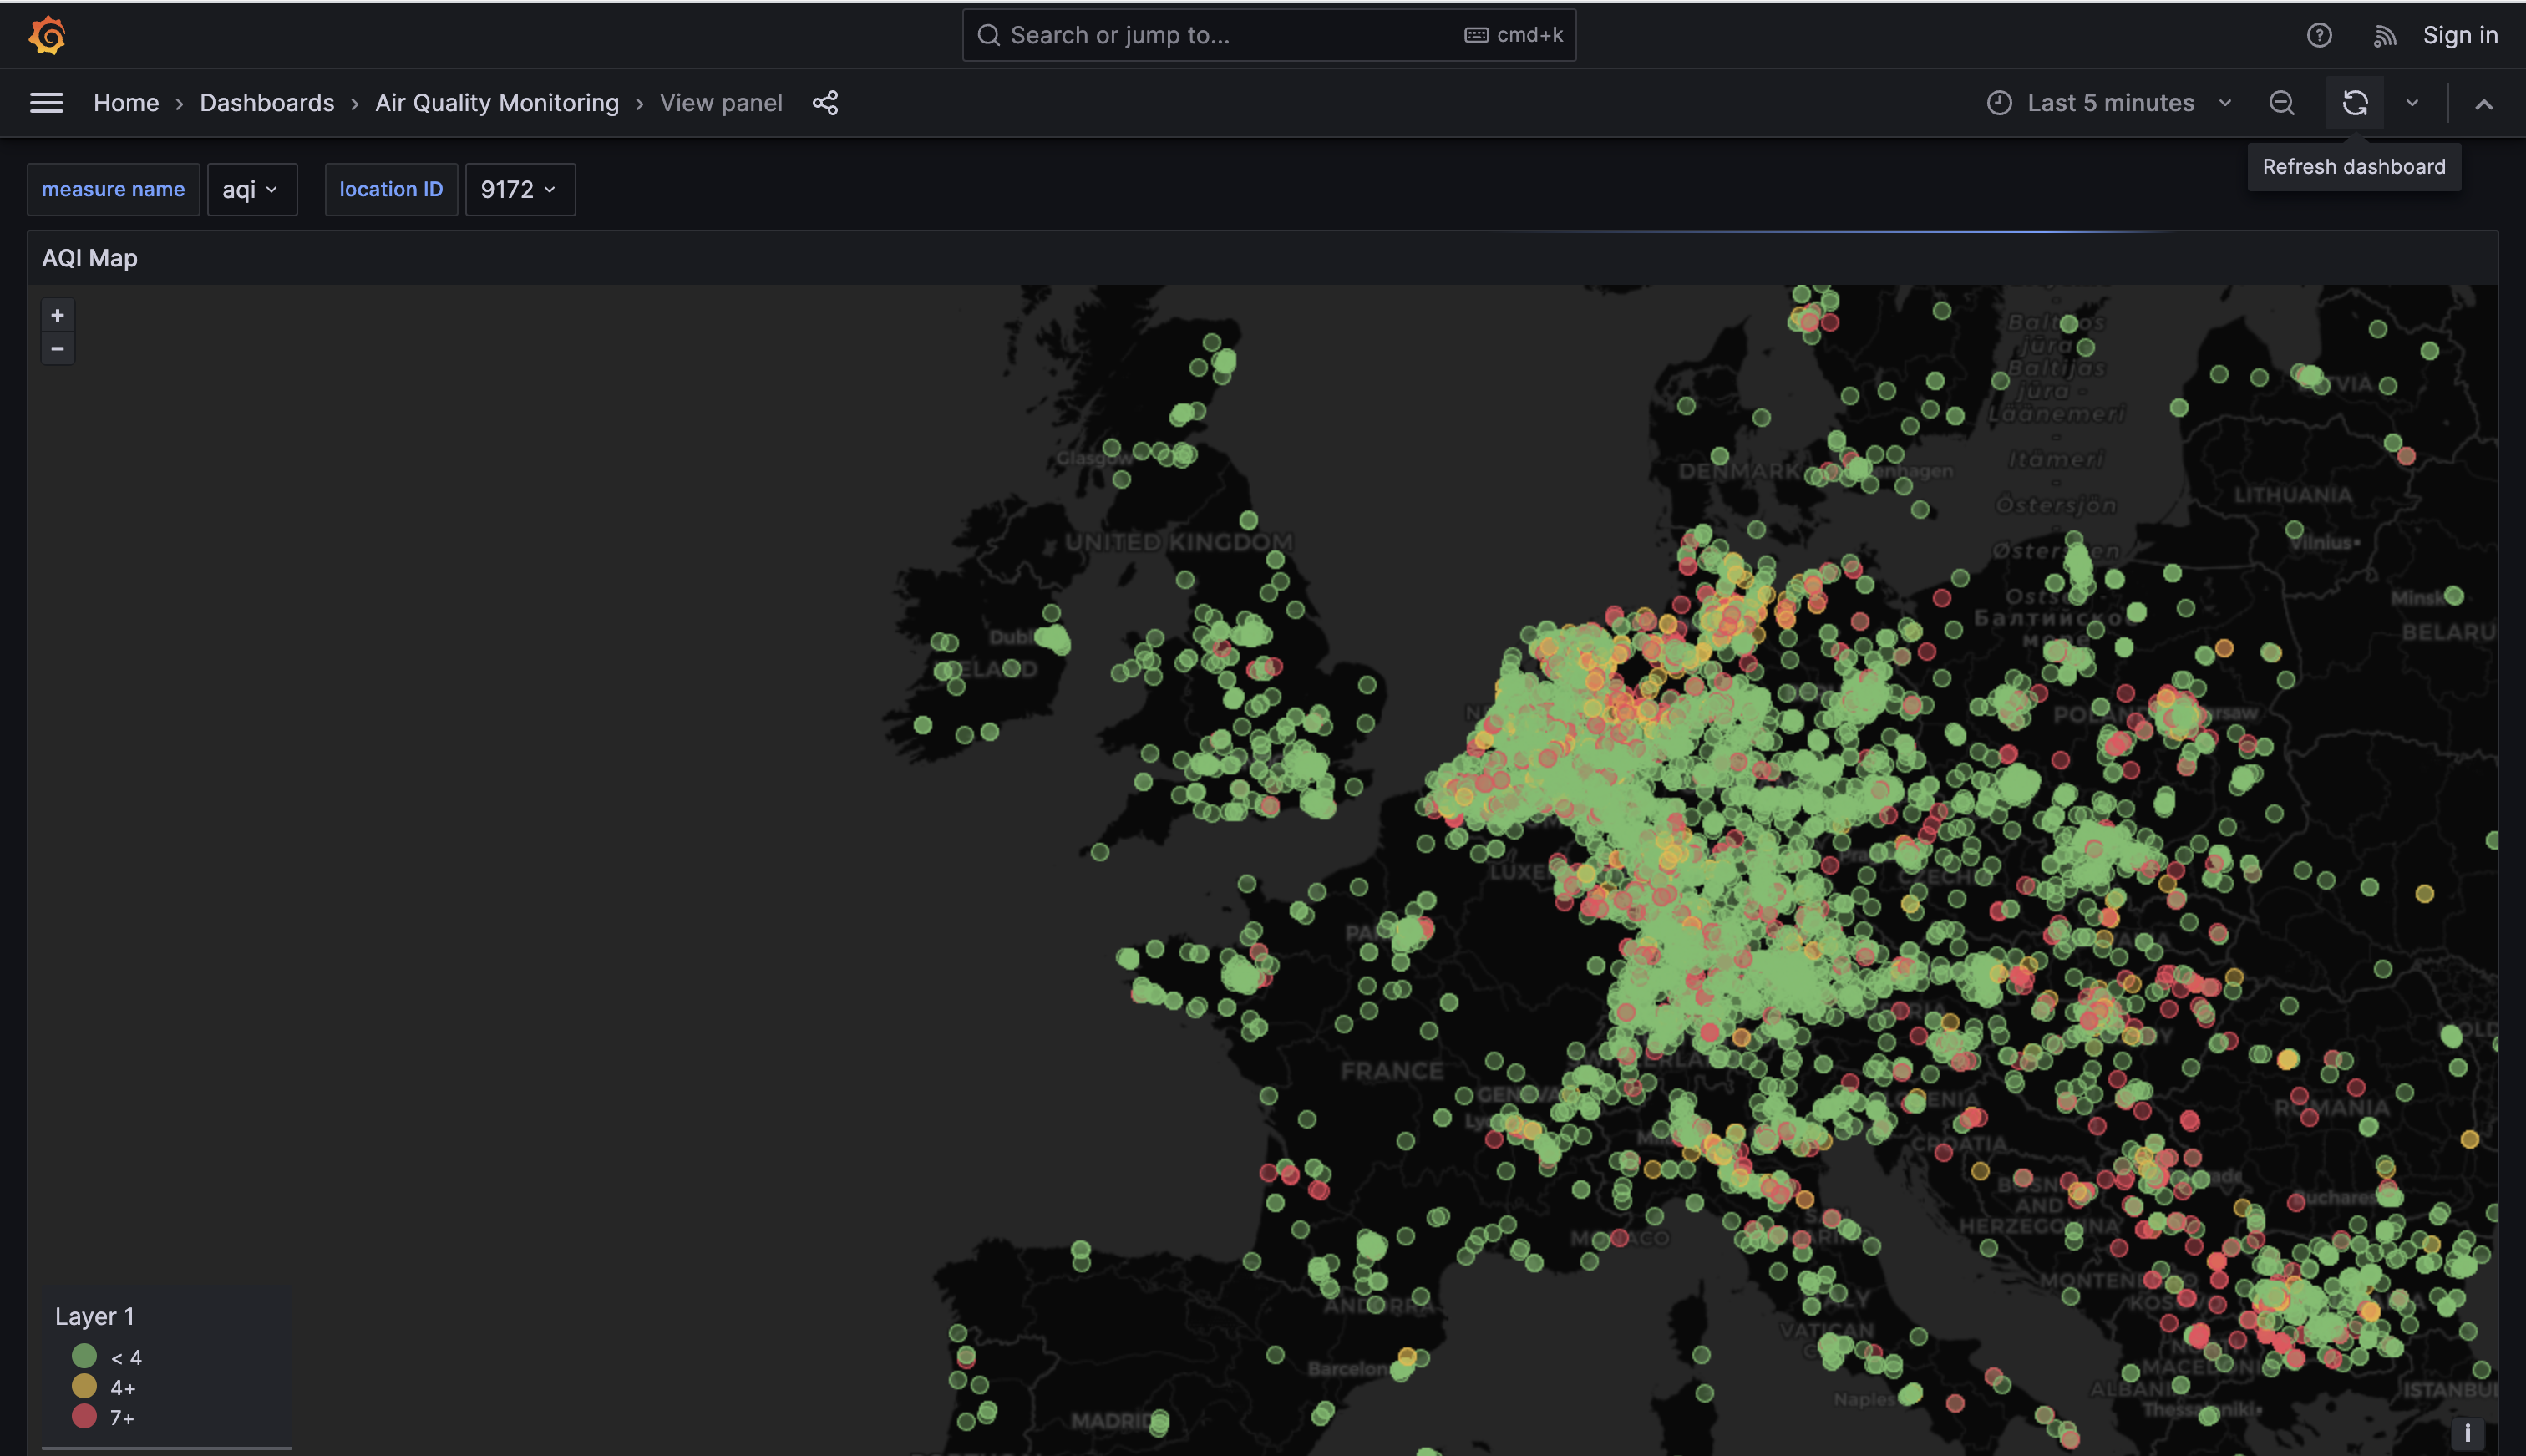
\includegraphics[width=1\linewidth]{images/grafana-4.png}
    \caption{Grafana Dashboard AQI Map Panel}\label{fig:grafana-aqi-map-panel}
\end{figure}

As required, the Grafana dashboard enables users to customise the time
interval, as shown in Figure~\ref{fig:grafana-iot-data-panel-time-range}.
\begin{figure}[H]
    \centering
    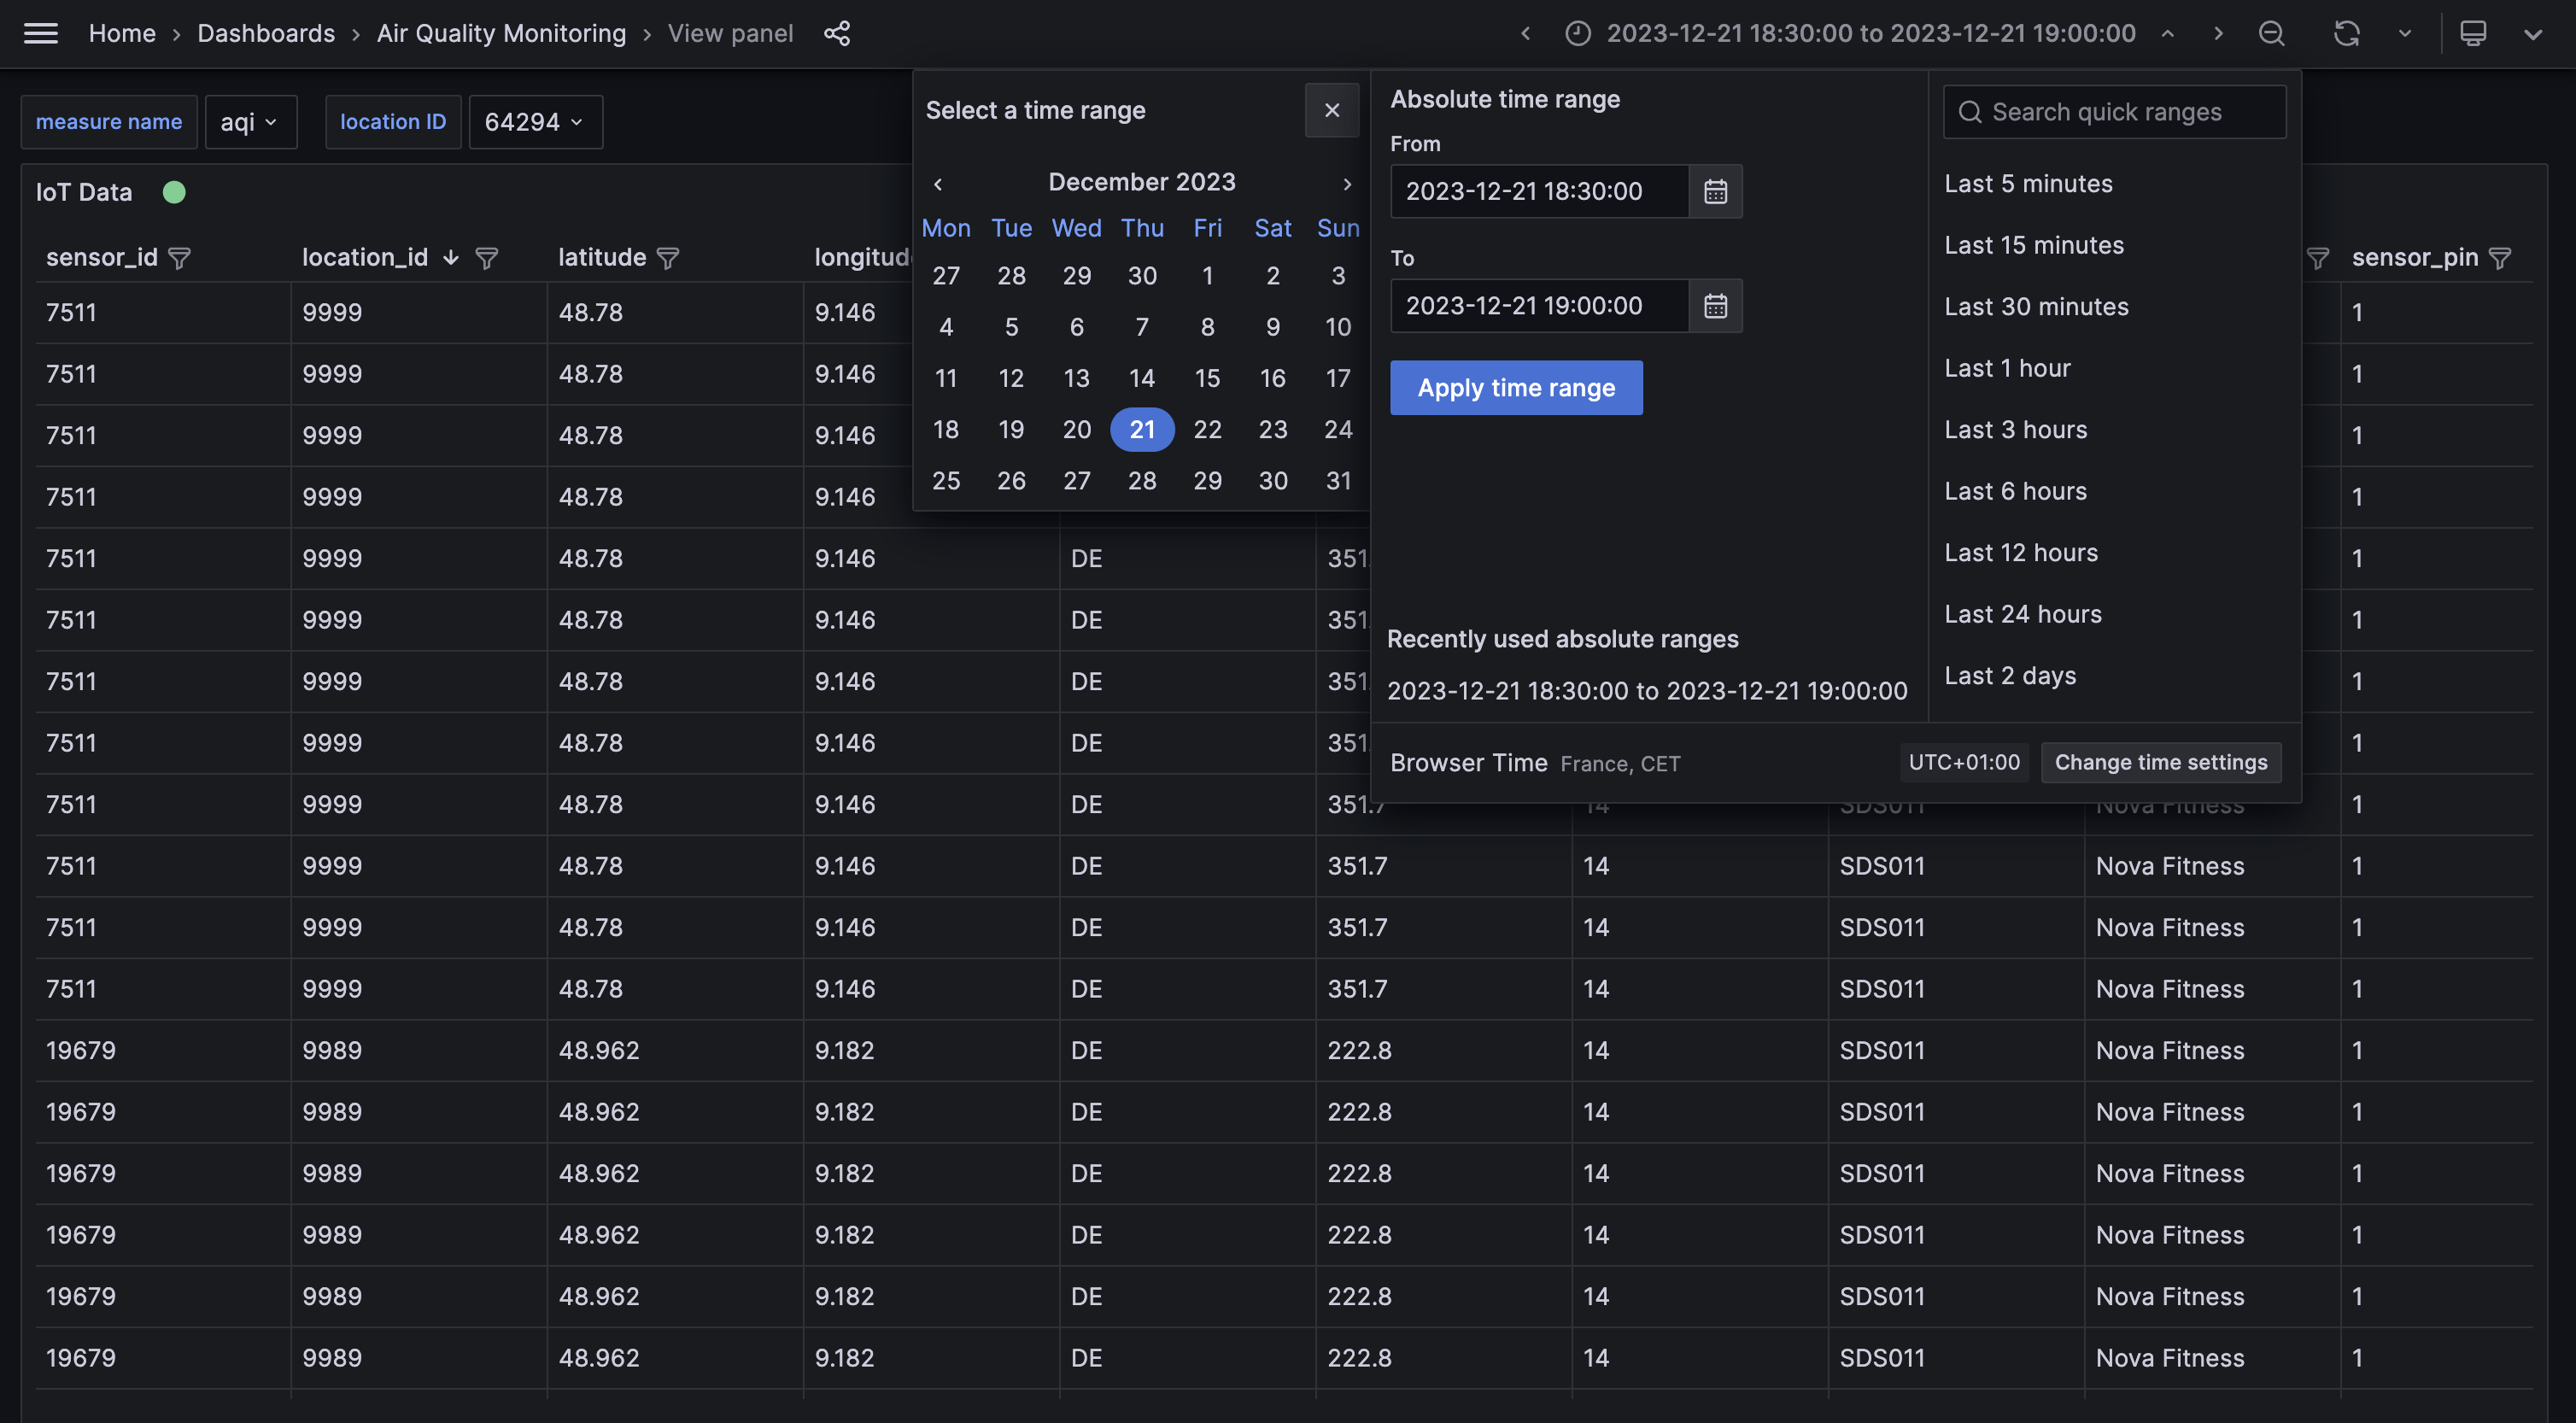
\includegraphics[width=1\linewidth]{images/time-range.png}
    \caption{Grafana Dashboard IoT Data Panel - Time Range Choice}\label{fig:grafana-iot-data-panel-time-range}
\end{figure}

\newpage
It is also possible to choose the measure value to display in the IoT Data panel, as shown in Figure~\ref{fig:grafana-iot-data-panel-measure-value}.
\begin{figure}[H]
    \centering
    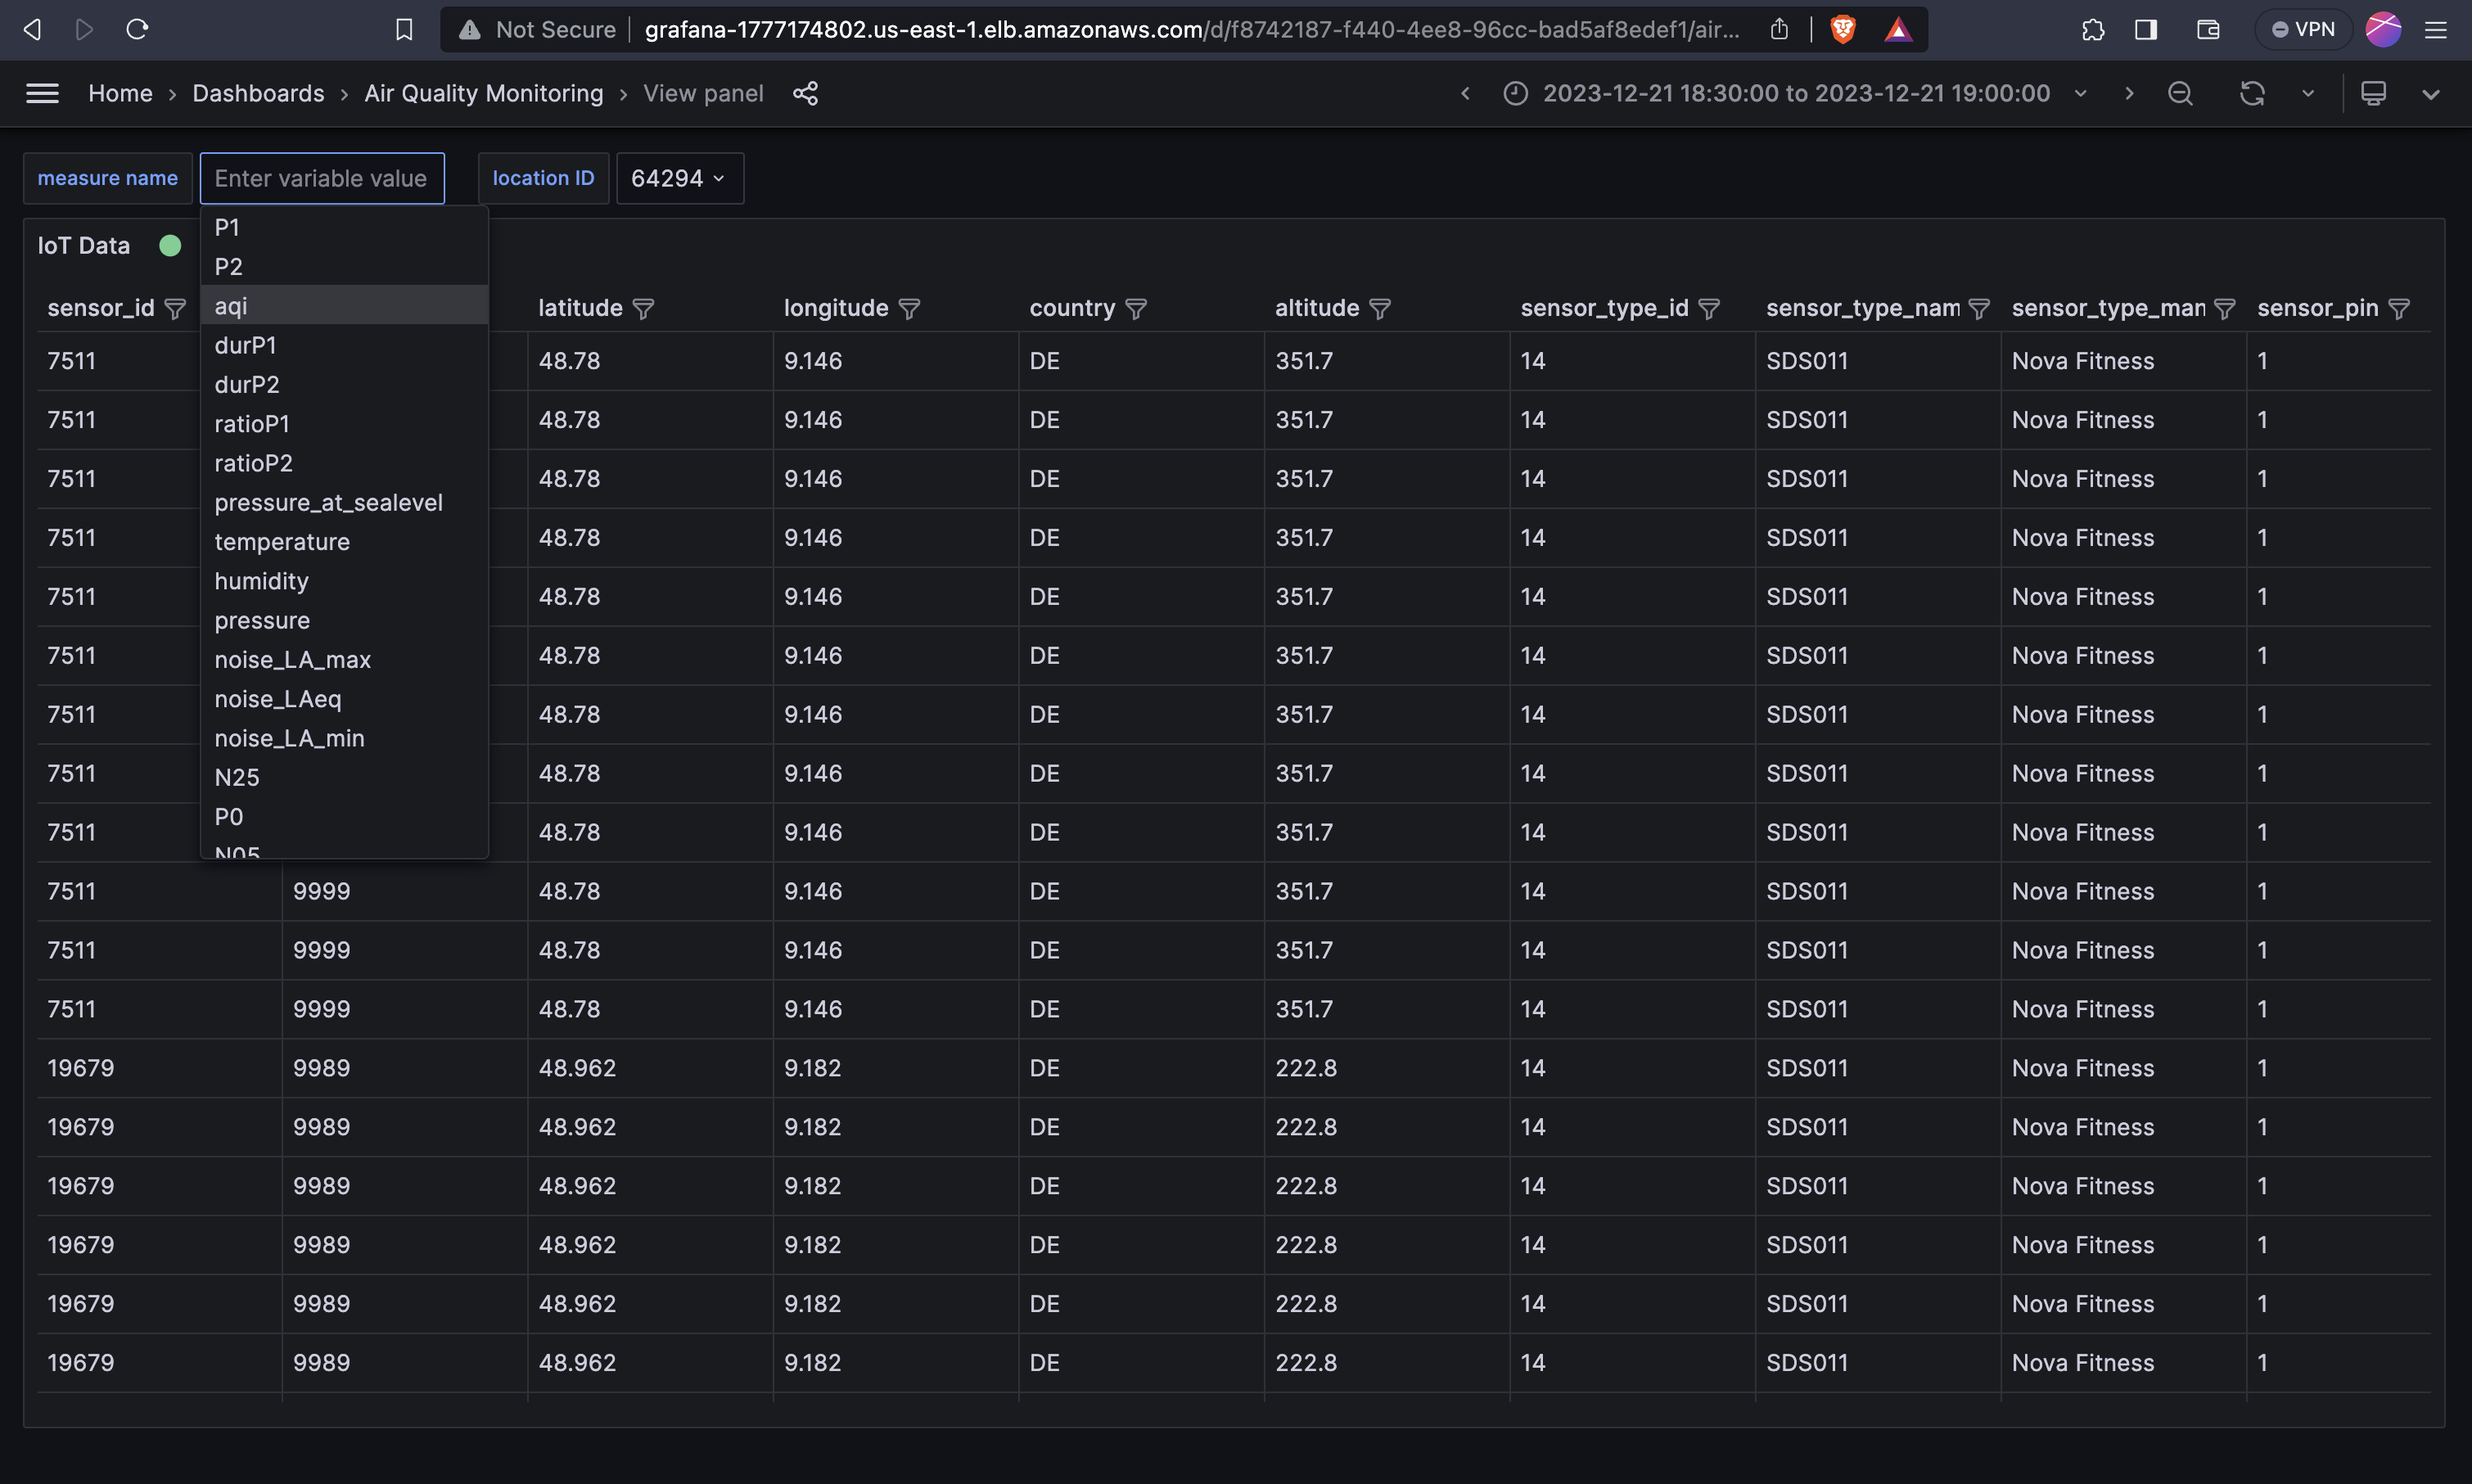
\includegraphics[width=1\linewidth]{images/measure-value.png}
    \caption{Grafana Dashboard IoT Data Panel - Measure Value Choice}\label{fig:grafana-iot-data-panel-measure-value}
\end{figure}

Moreove, it is possible to apply a filter to the data displayed in the IoT Data
panel. This can be done by clicking on the funnel icon, as shown in
Figure~\ref{fig:grafana-iot-data-panel-filter}.
\begin{figure}[H]
    \centering
    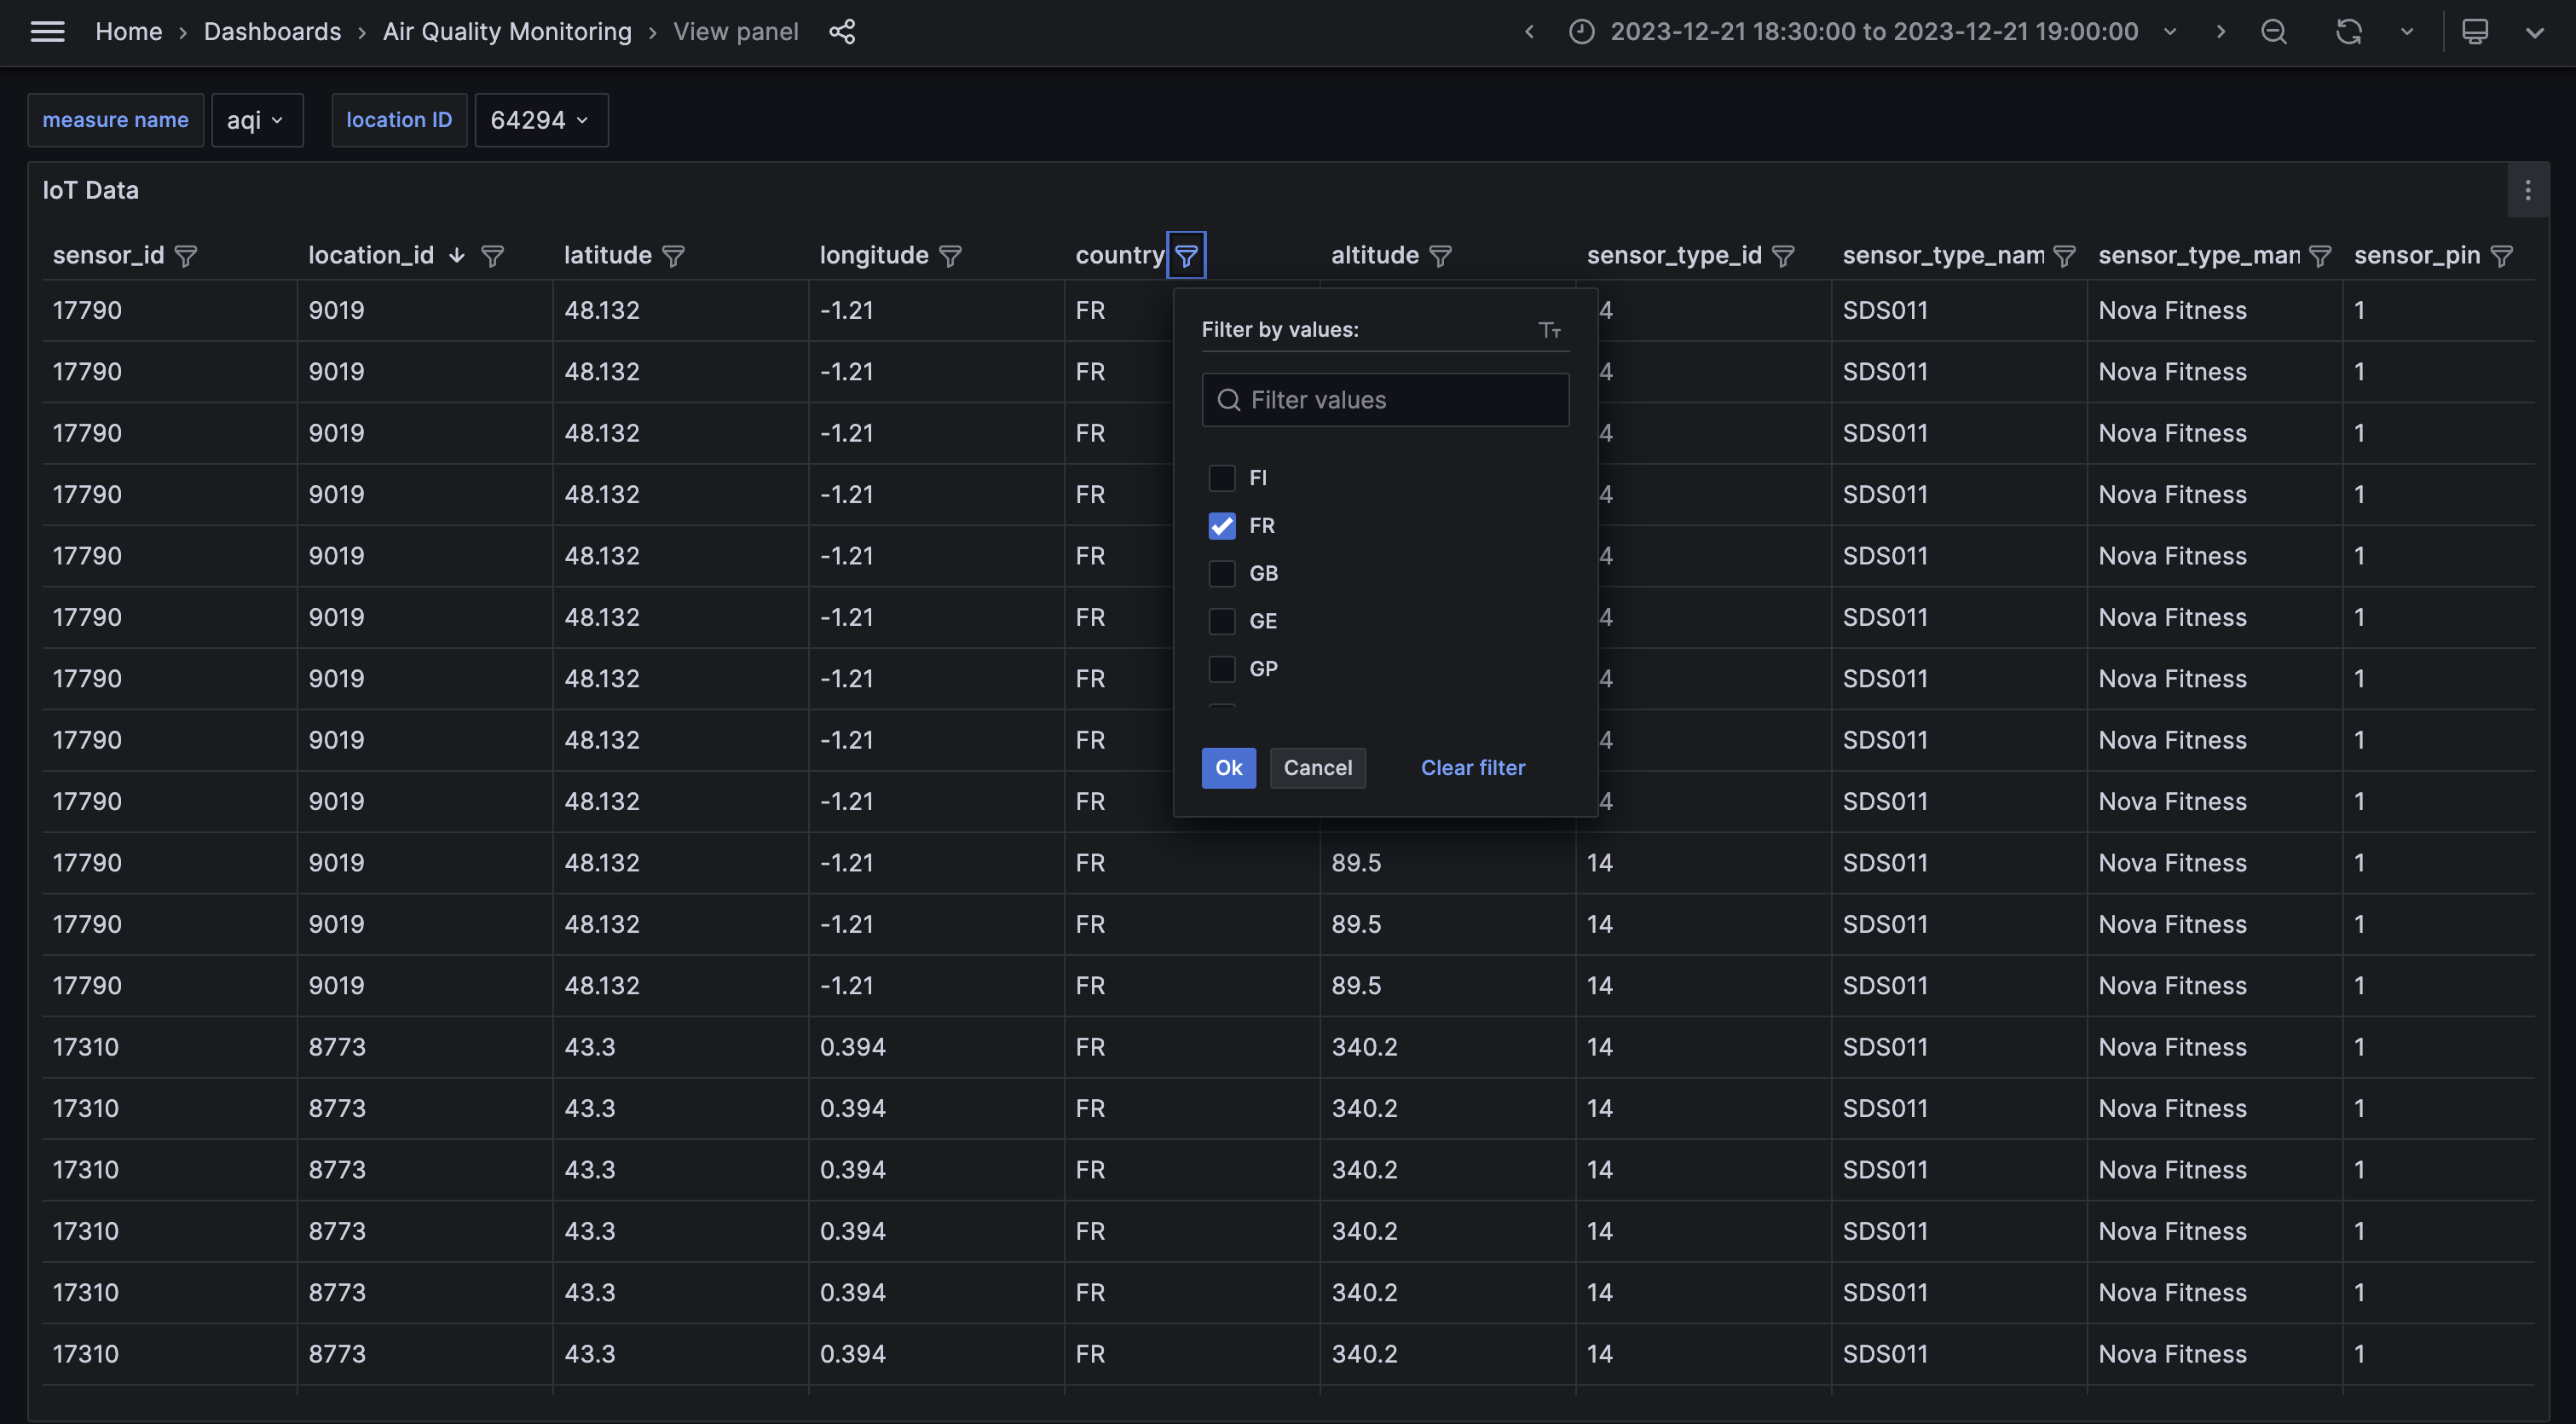
\includegraphics[width=1\linewidth]{images/filter.png}
    \caption{Grafana Dashboard IoT Data Panel - Apply a Filter}\label{fig:grafana-iot-data-panel-filter}
\end{figure}

\newpage
In addition, it is possible to export the data displayed in the IoT Data panel to a CSV file. This can be done by clicking on the \texttt{Download CSV} button, as shown in Figure~\ref{fig:grafana-iot-data-panel-export}.
\begin{figure}[H]
    \centering
    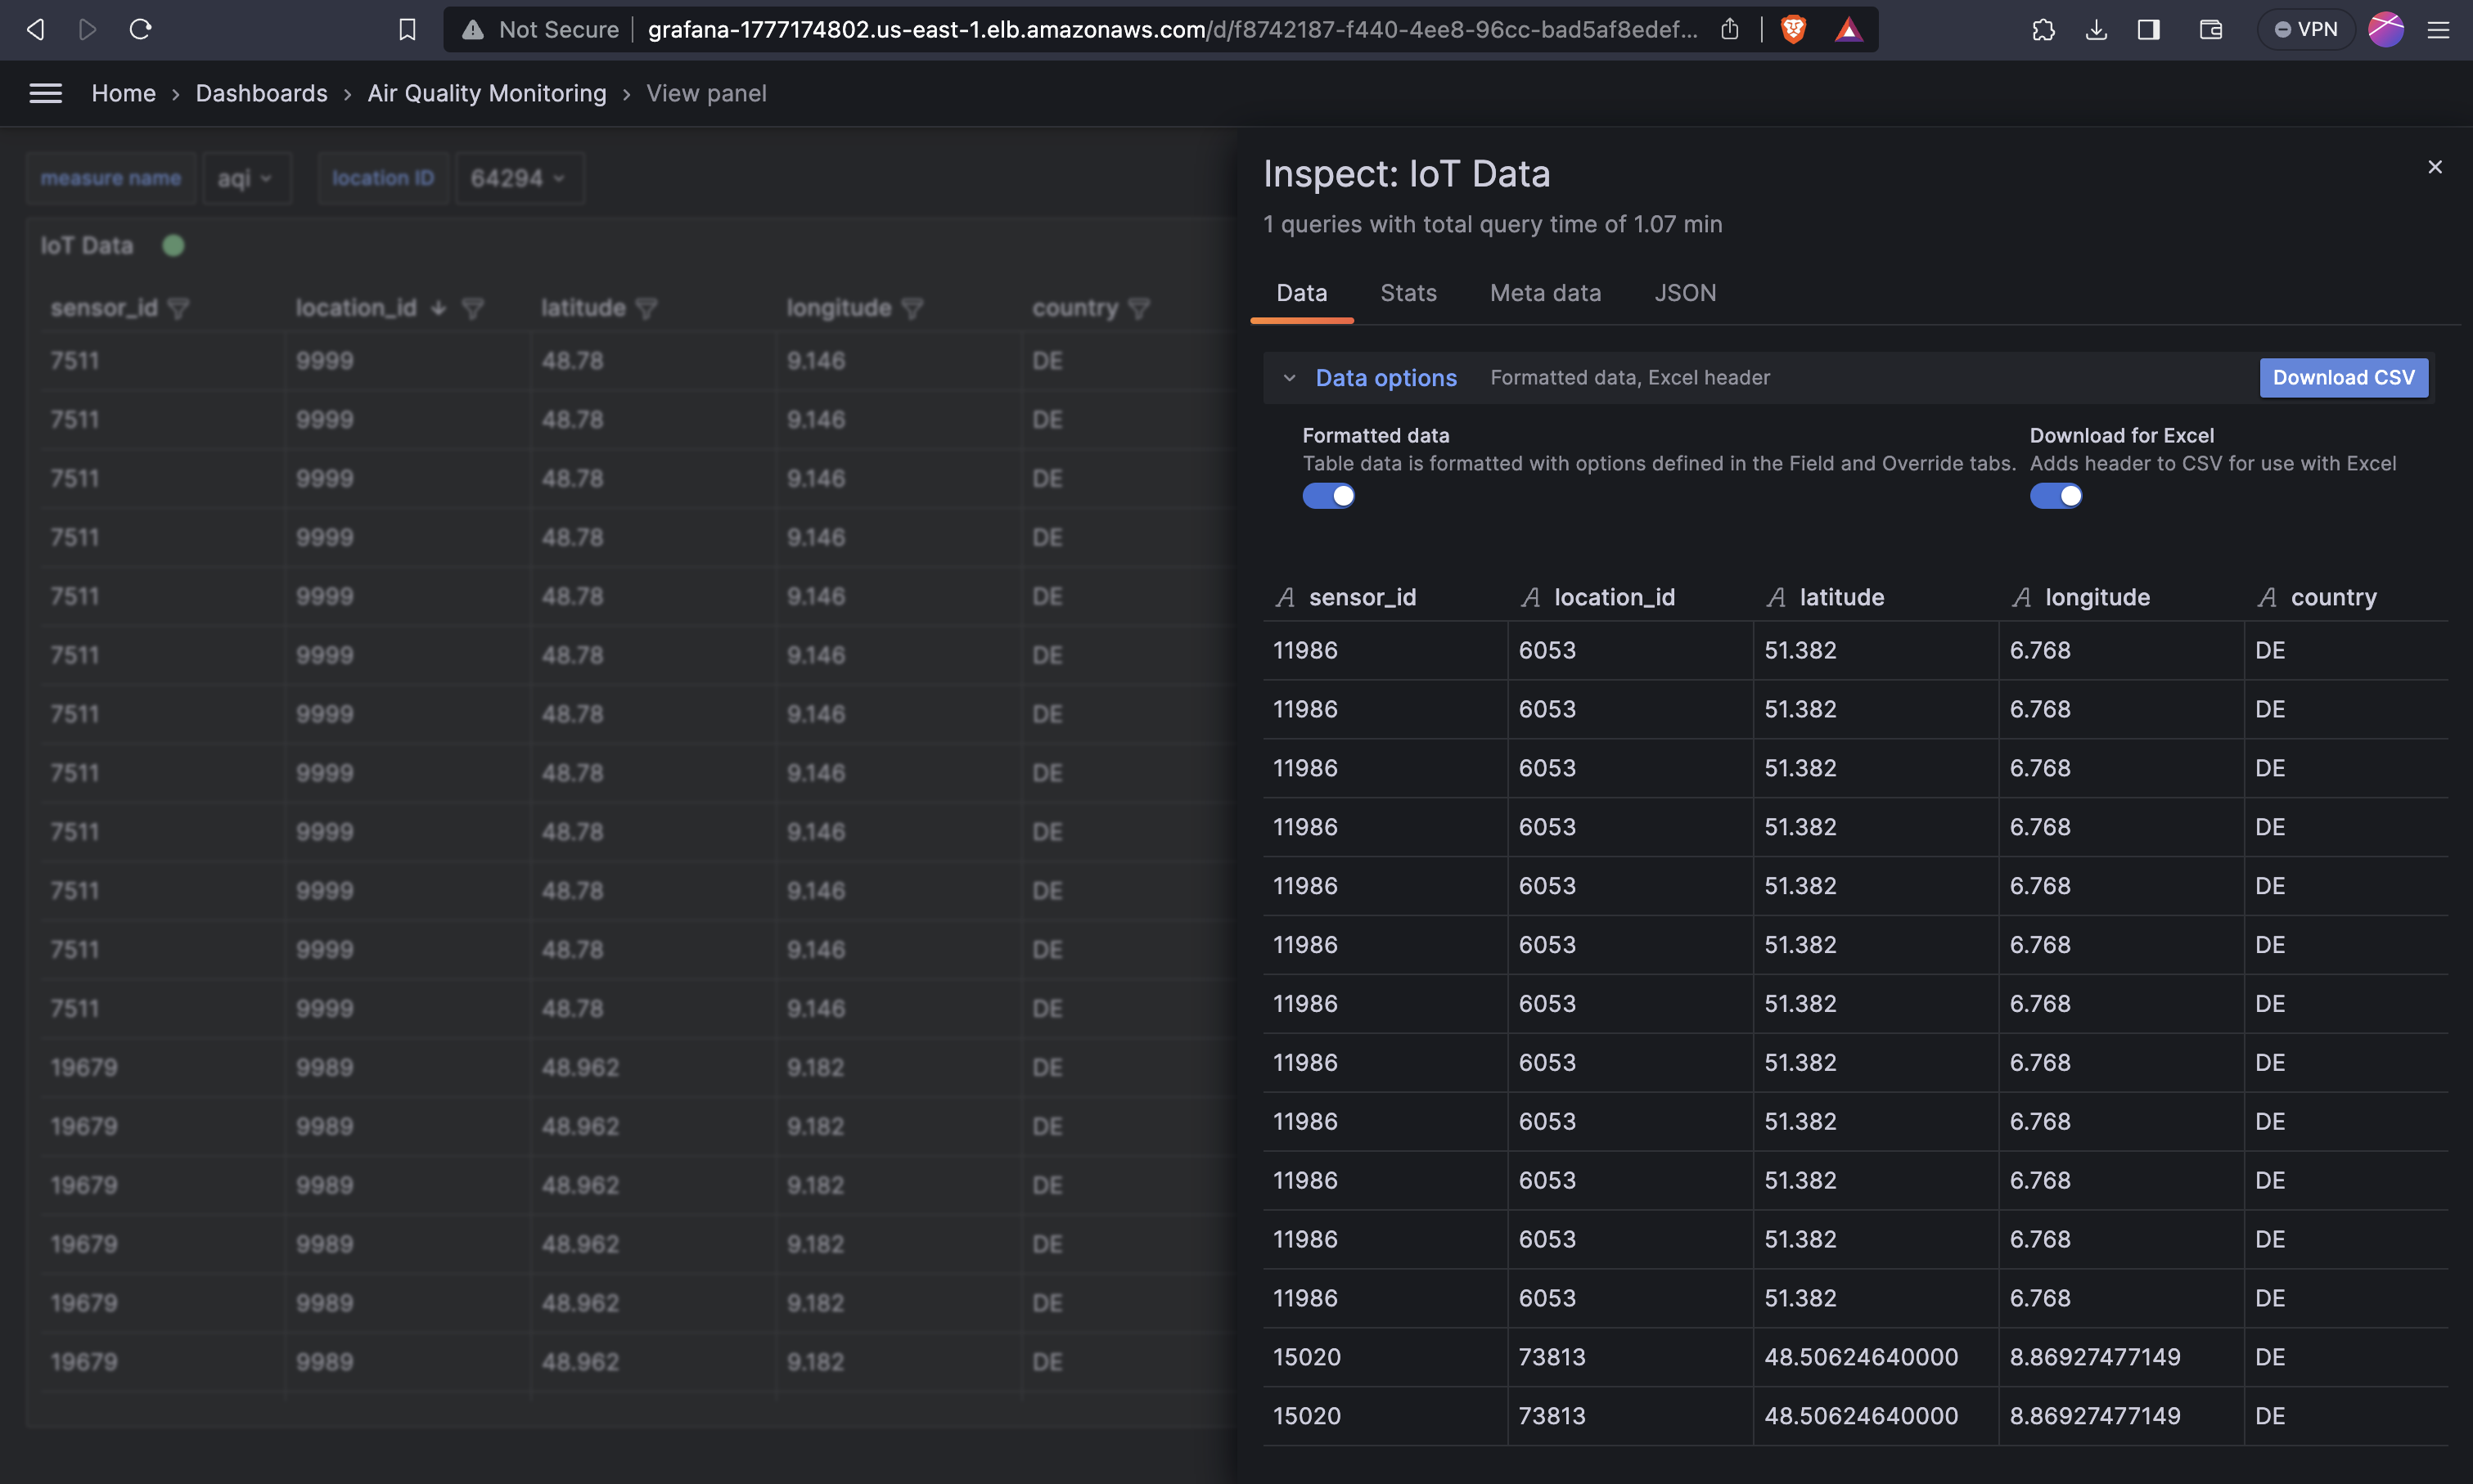
\includegraphics[width=1\linewidth]{images/export-2.png}
    \caption{Grafana Dashboard IoT Data Panel - Export Values}\label{fig:grafana-iot-data-panel-export}
\end{figure}

\newpage
\subsection{Load Test}
In order to test the scalability of the system, a load test was performed using
the Artillery load testing tool. The test consisted in simulating an increasing
number of customers consuming the grafana dashboards simultaneously, to
demonstrate the elasticity of the solution developed. The results of the test
are shown in Figure~\ref{fig:load-test-result}.

\subsubsection{Artillery Load Test}
The load test was performed using the Artillery load testing script available
in Appendix~\ref{appendix:artillery-load-test}. Here are the steps of the load
test:
\begin{enumerate}
    \item \textbf{Stage 1:} 1 new user is added every second for 50 seconds.
    \item \textbf{Pause:} No new users are added for 30 seconds.
    \item \textbf{Stage 2:} 1 new user is added every second for 60 seconds.
    \item \textbf{Pause:} No new users are added for 60 seconds.
    \item \textbf{Stage 3:} 1 new user is added every second for 60 seconds.
    \item \textbf{Pause:} No new users are added for 30 seconds.
    \item \textbf{Stage 4:} 2 new users are added every second for 50 seconds.
    \item \textbf{Pause:} No new users are added for 60 seconds.
    \item \textbf{Stage 5:} 2 new users are added every second for 60 seconds.
    \item \textbf{Pause:} No new users are added for 60 seconds.
    \item \textbf{Stage 6:} 2 new users are added every second for 80 seconds.
\end{enumerate}
Each user is configured to access 2 endpoints of the Grafana dashboard 100 times. Besides, this test was performed several times to ensure the reliability of the results.

\subsubsection{Auto Scaling Group Behaviour Monitoring}
The Auto Scaling Group behaviour was monitored during the load test thanks to a
Python script available in Appendix~\ref{appendix:monitoring}. The monitoring
data is available in the \texttt{metrics.csv} file in the \texttt{test} folder.
For enhanced data interpretation and visualisation, a Jupyter Notebook was
developed to provide a graphical representation of system performance during
load testing, as shown in Figure~\ref{fig:load-test-result}, which illustrates
the dynamic scaling actions triggered by fluctuating demand on system
resources.

At the start of the load test, only one instance was active. The data shows
that this instance quickly reached its processing capacity. In response, the
auto-scaling group launched additional instances, as evidenced by the
subsequent reductions in CPU usage after each new instance was integrated into
the service architecture. Once demand calmed and CPU utilisation fell below the
42\% threshold, the Auto Scaling Group effectively deprovisioned the excess
instances. This strategic downscaling is essential to optimise resource
utilisation and cost management. The figure highlights the elasticity of the
system, with the Auto Scaling Group skilfully modulating the number of active
instances according to the real-time workload, maintaining system stability and
performance efficiency.

\begin{figure}[H]
    \centering
    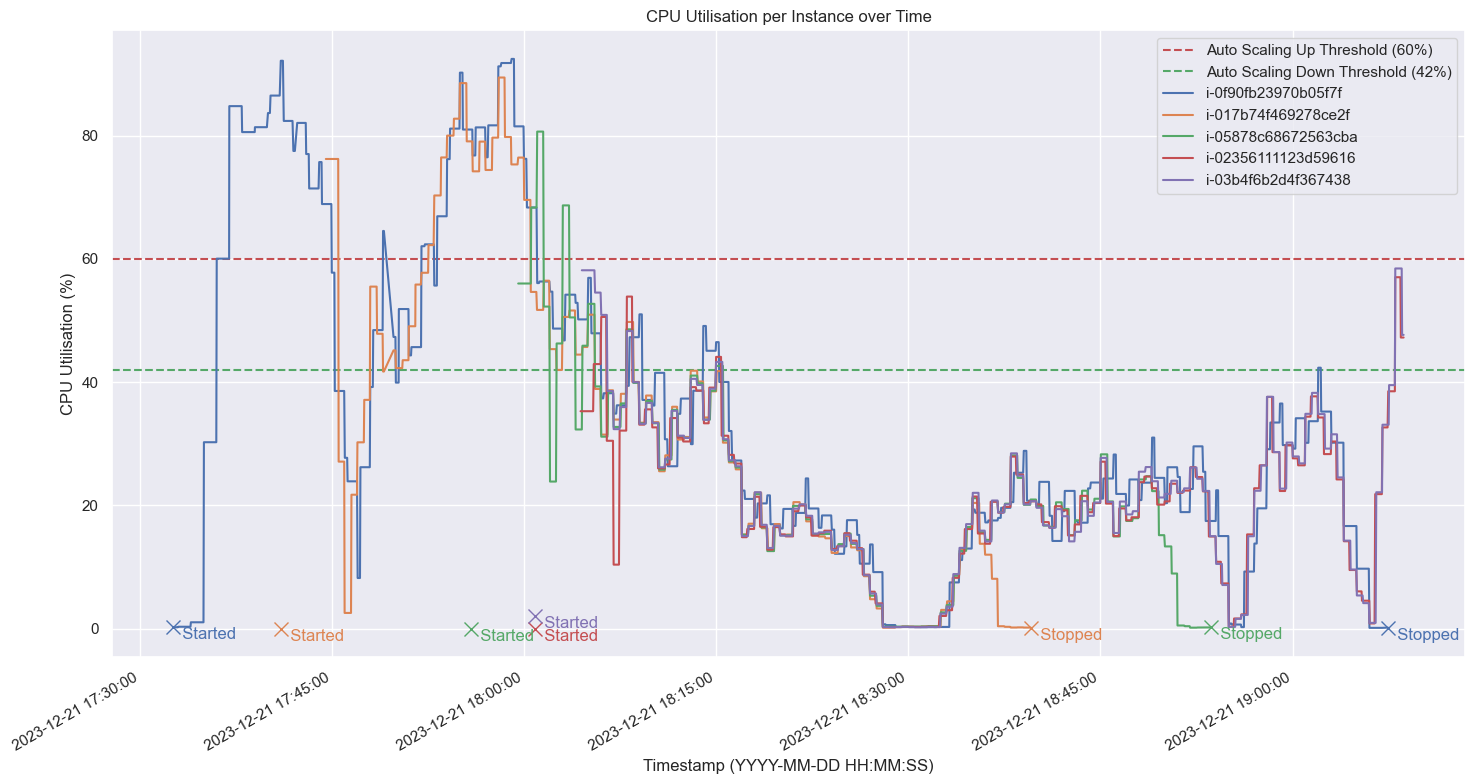
\includegraphics[width=1\linewidth]{images/autoscaling-test.png}
    \caption{Load Test Result}\label{fig:load-test-result}
\end{figure}

\newpage
\section{Data Security and Sovereignty Considerations}
Data security and sovereignty are critical elements in managing environmental
sensor data, reflecting the importance of addressing evolving threats and
protection mechanisms in IoT as highlighted in recent research.

\subsection{Data Security}
Data security for environmental sensors involves protecting sensitive data from
unauthorised access, alteration, theft or destruction. The integration of IoT
devices into wider networks introduces unique vulnerabilities. It is imperative
to secure these devices against cyber threats, ensuring that the data they
transmit and their operational integrity are protected. This includes
protecting devices, their firmware and the networks to which they connect from
unauthorised access and cyber attacks~\cite{CurrentResearchIoTSecurity2020}.

In addition to device and network security, managing the vast volumes of data
generated by these sensors is crucial. The use of cloud-based solutions offers
scalability and flexibility, but also raises significant security issues. The
implementation of secure data transfer mechanisms, encrypted storage solutions
and regular vulnerability assessments are essential to preserve data integrity
and confidentiality. Compliance with international security standards and best
practice ensures that data storage and processing meet the highest levels of
security.

\subsection{Data Sovereignty}
Data sovereignty concerns the legal and regulatory aspects of data management,
particularly with regard to the geographical location of data. The
transnational nature of IoT deployments requires a thorough understanding of
the various international and regional laws governing data privacy and
protection. For example, the physical location of servers may subject data to
the legal jurisdiction of that country, which affects the level of data
protection and compliance obligations.

In addition, the transmission and processing of data across borders must comply
with international data protection agreements, such as the General Data
Protection Regulation (GDPR) in the European Union. This includes ensuring that
data flows comply with the legal requirements of all countries involved.

Organisations need to navigate these complex legal landscapes while maintaining
data accessibility and control. In cases where data crosses international
borders, it is essential to understand who has jurisdiction over the data and
under what conditions it can be accessed or shared. This is particularly
important in situations involving judicial investigations or government
requests for access to data.

\newpage
\chapter{Conclusion}
To conclude, this project successfully demonstrated the integration of cloud
computing and IoT technologies to create a robust real-time environmental
monitoring system, focusing on air quality. The implementation of a scalable
data processing pipeline using Apache Spark and Amazon Timestream enabled the
efficient management and analysis of large volumes of sensor data, ensuring
accurate real-time AQI calculations. The development of a user-friendly Grafana
dashboard facilitated data visualisation and accessibility, making the system
invaluable to stakeholders in environmental monitoring, public health and urban
planning. Load tests confirmed the system's scalability and responsiveness,
underlining its ability to adapt dynamically to varying demands. Compliance
with data security and sovereignty standards has ensured that the system
complies with international regulations. This project not only demonstrates the
practical application of combining cloud computing and IoT in environmental
data management, but also lays the foundations for future advances in this
vital area.

\bibliographystyle{CranfieldNumbered}
\bibliography{CUCitations}

\appendix
\chapter{Documentation}

\begin{subappendices}
    \section{Project tree}
    \begin{lstlisting}[breaklines=true, basicstyle=\small]
    lib/
        collecting.py
        processing.py
        storing.py
    scripts/
        get_iam_credentials.sh
        start_spark_job.sh
    services/
        get_iam_credentials.service
        spark_python_job.service
    test/
        artillery_load_test.yml
        monitoring.py
        metrics.csv
        results.json
        visualisation_load_test.ipynb
    main.py
    README.md
    requirements.txt
    \end{lstlisting}

    \section{Getting Started}
    To run the program, follow these steps:
    \begin{enumerate}
        \itemindent=17.87pt
        \item Create a virtual environment using \texttt{python3 -m venv venv}.
        \item Activate the virtual environment using \texttt{source venv/bin/activate}.
        \item Install the required dependencies using \texttt{pip3 install -r
                  requirements.txt}.
        \item Run the program using \texttt{python3 main.py}.
        \item Visualise the results using \texttt{visualisation.ipynb} (Jupyter Notebook).
    \end{enumerate}

    \section{Detailed Features of Functions}
    \begin{description}
        \item \texttt{collecting.py}
              \begin{itemize}
                  \item \texttt{fetch\_sensors\_data(sparkSession)}: Function to ingest the latest data from the sensors and returns it as a Spark DataFrame.
              \end{itemize}

        \item \texttt{processing.py}
              \begin{itemize}
                  \item \texttt{get\_aqi\_value\_p25(value)}: Function for calculating the AQI value for PM2.5.
                  \item \texttt{get\_aqi\_value\_p10(value)}: Function for calculating the AQI value for PM10.
                  \item \texttt{computeAQI(df)}: Function for calculating the AQI value for each particulate matter sensor and returning the DataFrame with the AQI column.
              \end{itemize}

        \item \texttt{storing.py}
              \begin{itemize}
                  \item \texttt{keepOnlyUpdatedRows(database\_name, table\_name, df)}: Function for keeping only the rows that have been updated in the DataFrame.
                  \item \texttt{\_print\_rejected\_records\_exceptions(err)}: Internal function for printing the rejected records exceptions.
                  \item \texttt{write\_records(database\_name, table\_name, client, records)}: Internal function for writing a batch of records to the Timestream database.
                  \item \texttt{writeToTimestream(database\_name, table\_name, partionned\_df)}: Function for writing the DataFrame to the Timestream database.
              \end{itemize}
    \end{description}
\end{subappendices}

\chapter{Source Codes}
\begin{subappendices}
    \section{Ingestion, Processing \& Storing Pipeline Source Code}\label{appendix:main}
    \lstinputlisting[style=pythonstyle]{../main.py}

    \newpage
    \section{Data Collecting Source Code}\label{appendix:collecting}
    \lstinputlisting[style=pythonstyle]{../lib/collecting.py}

    \newpage
    \section{Data Processing Source Code}\label{appendix:processing}
    \lstinputlisting[style=pythonstyle]{../lib/processing.py}

    \newpage
    \section{Data Storing Source Code}\label{appendix:storing}
    \lstinputlisting[style=pythonstyle]{../lib/storing.py}

    \newpage
    \section{Scripts \& Services Source Codes }
    \subsection{Scripts}

    \subsubsection{Get IAM Credentials Script}
    Script used by the \texttt{get\_iam\_credentials} service to retrieve the IAM
    credentials from the metadata server.\label{appendix:get-iam-credentials}
    \lstinputlisting[style=bashstyle]{../scripts/get_iam_credentials.sh}

    \subsubsection{Start Spark Job Script}
    Script used by the \texttt{spark\_python\_job} service to run the Python Spark
    job.\label{appendix:start-spark-job}
    \lstinputlisting[style=bashstyle]{../scripts/start_spark_job.sh}

    \newpage
    \subsection{Services}

    \subsubsection{Get IAM Credentials Service}
    Service used by the Ubuntu EC2 instance to retrieve the IAM credentials from
    the metadata server.\label{appendix:get-iam-credentials-service}
    \lstinputlisting[style=servicestyle]{../services/get_iam_credentials.service}

    \subsubsection{Spark Python Job Service}
    Service used by the Ubuntu EC2 instance to run the Python Spark job (Data
    Collecting, Processing and Storing).\label{appendix:spark-python-job-service}
    \lstinputlisting[style=servicestyle]{../services/spark_python_job.service}

    \newpage
    \section{Load Test Source Codes }

    \subsection{Artillery Load Test Configuration File}\label{appendix:artillery-load-test}
    \lstinputlisting[style=ymlstyle]{../test/artillery_load_test.yml}

    \newpage
    \subsection{Instances Monitoring Script}\label{appendix:monitoring}
    \lstinputlisting[style=pythonstyle]{../test/monitoring.py}
\end{subappendices}

\end{document}

